\documentclass[a4paper,12pt]{article}
\usepackage[utf8]{inputenc}
\usepackage[french]{babel}
\usepackage[T1]{fontenc}
\usepackage[top=2cm,bottom=2cm,left=2cm,right=2cm]{geometry}
\usepackage{graphicx}
\usepackage{wrapfig}
\usepackage{url}

\begin{document}

\begin{titlepage}
	\begin{center}
		\Large{Année universitaire 2016-2017}\\
		\Large{Université de Caen Basse-Normandie}\\[1cm]
		
		\huge{Rapport sur le deuxième semestre de TPA}\\
		\vspace{3cm}
		
		Alexis Carreau\\
		Thomas Lécluse\\
		Emma Mauger\\
		Théo Sarrazin\\
		
		\normalsize{\textit{ ~ L2 Informatique}}\\
		\medskip
		\vspace{2cm}
		
		\huge{\textbf{Réalisation d'un IDE en Python}}
		
	\end{center}
\end{titlepage}

\tableofcontents
\newpage

\section{Introduction}

	Voici un résumé de ce que nous avions à la fin du premier semestre.\\
	
	Notre IDE était capable d'ouvrir des documents avec l'extention .c ou .h à partir de projets qu'on avait créé. On pouvait ouvrir plusieurs documents, et avoir une liste d'onglets. Nous avions un navigateur de fichiers qui nous permettait de naviguer entre nos différents projets et leurs documents. Une barre de menu nous permettait d'accéder à nos différentes fonctionnalités, et on affichait à l'aide d'une barre de statut différents messages répondant aux requêtes de l'utilisateur.\\
	
	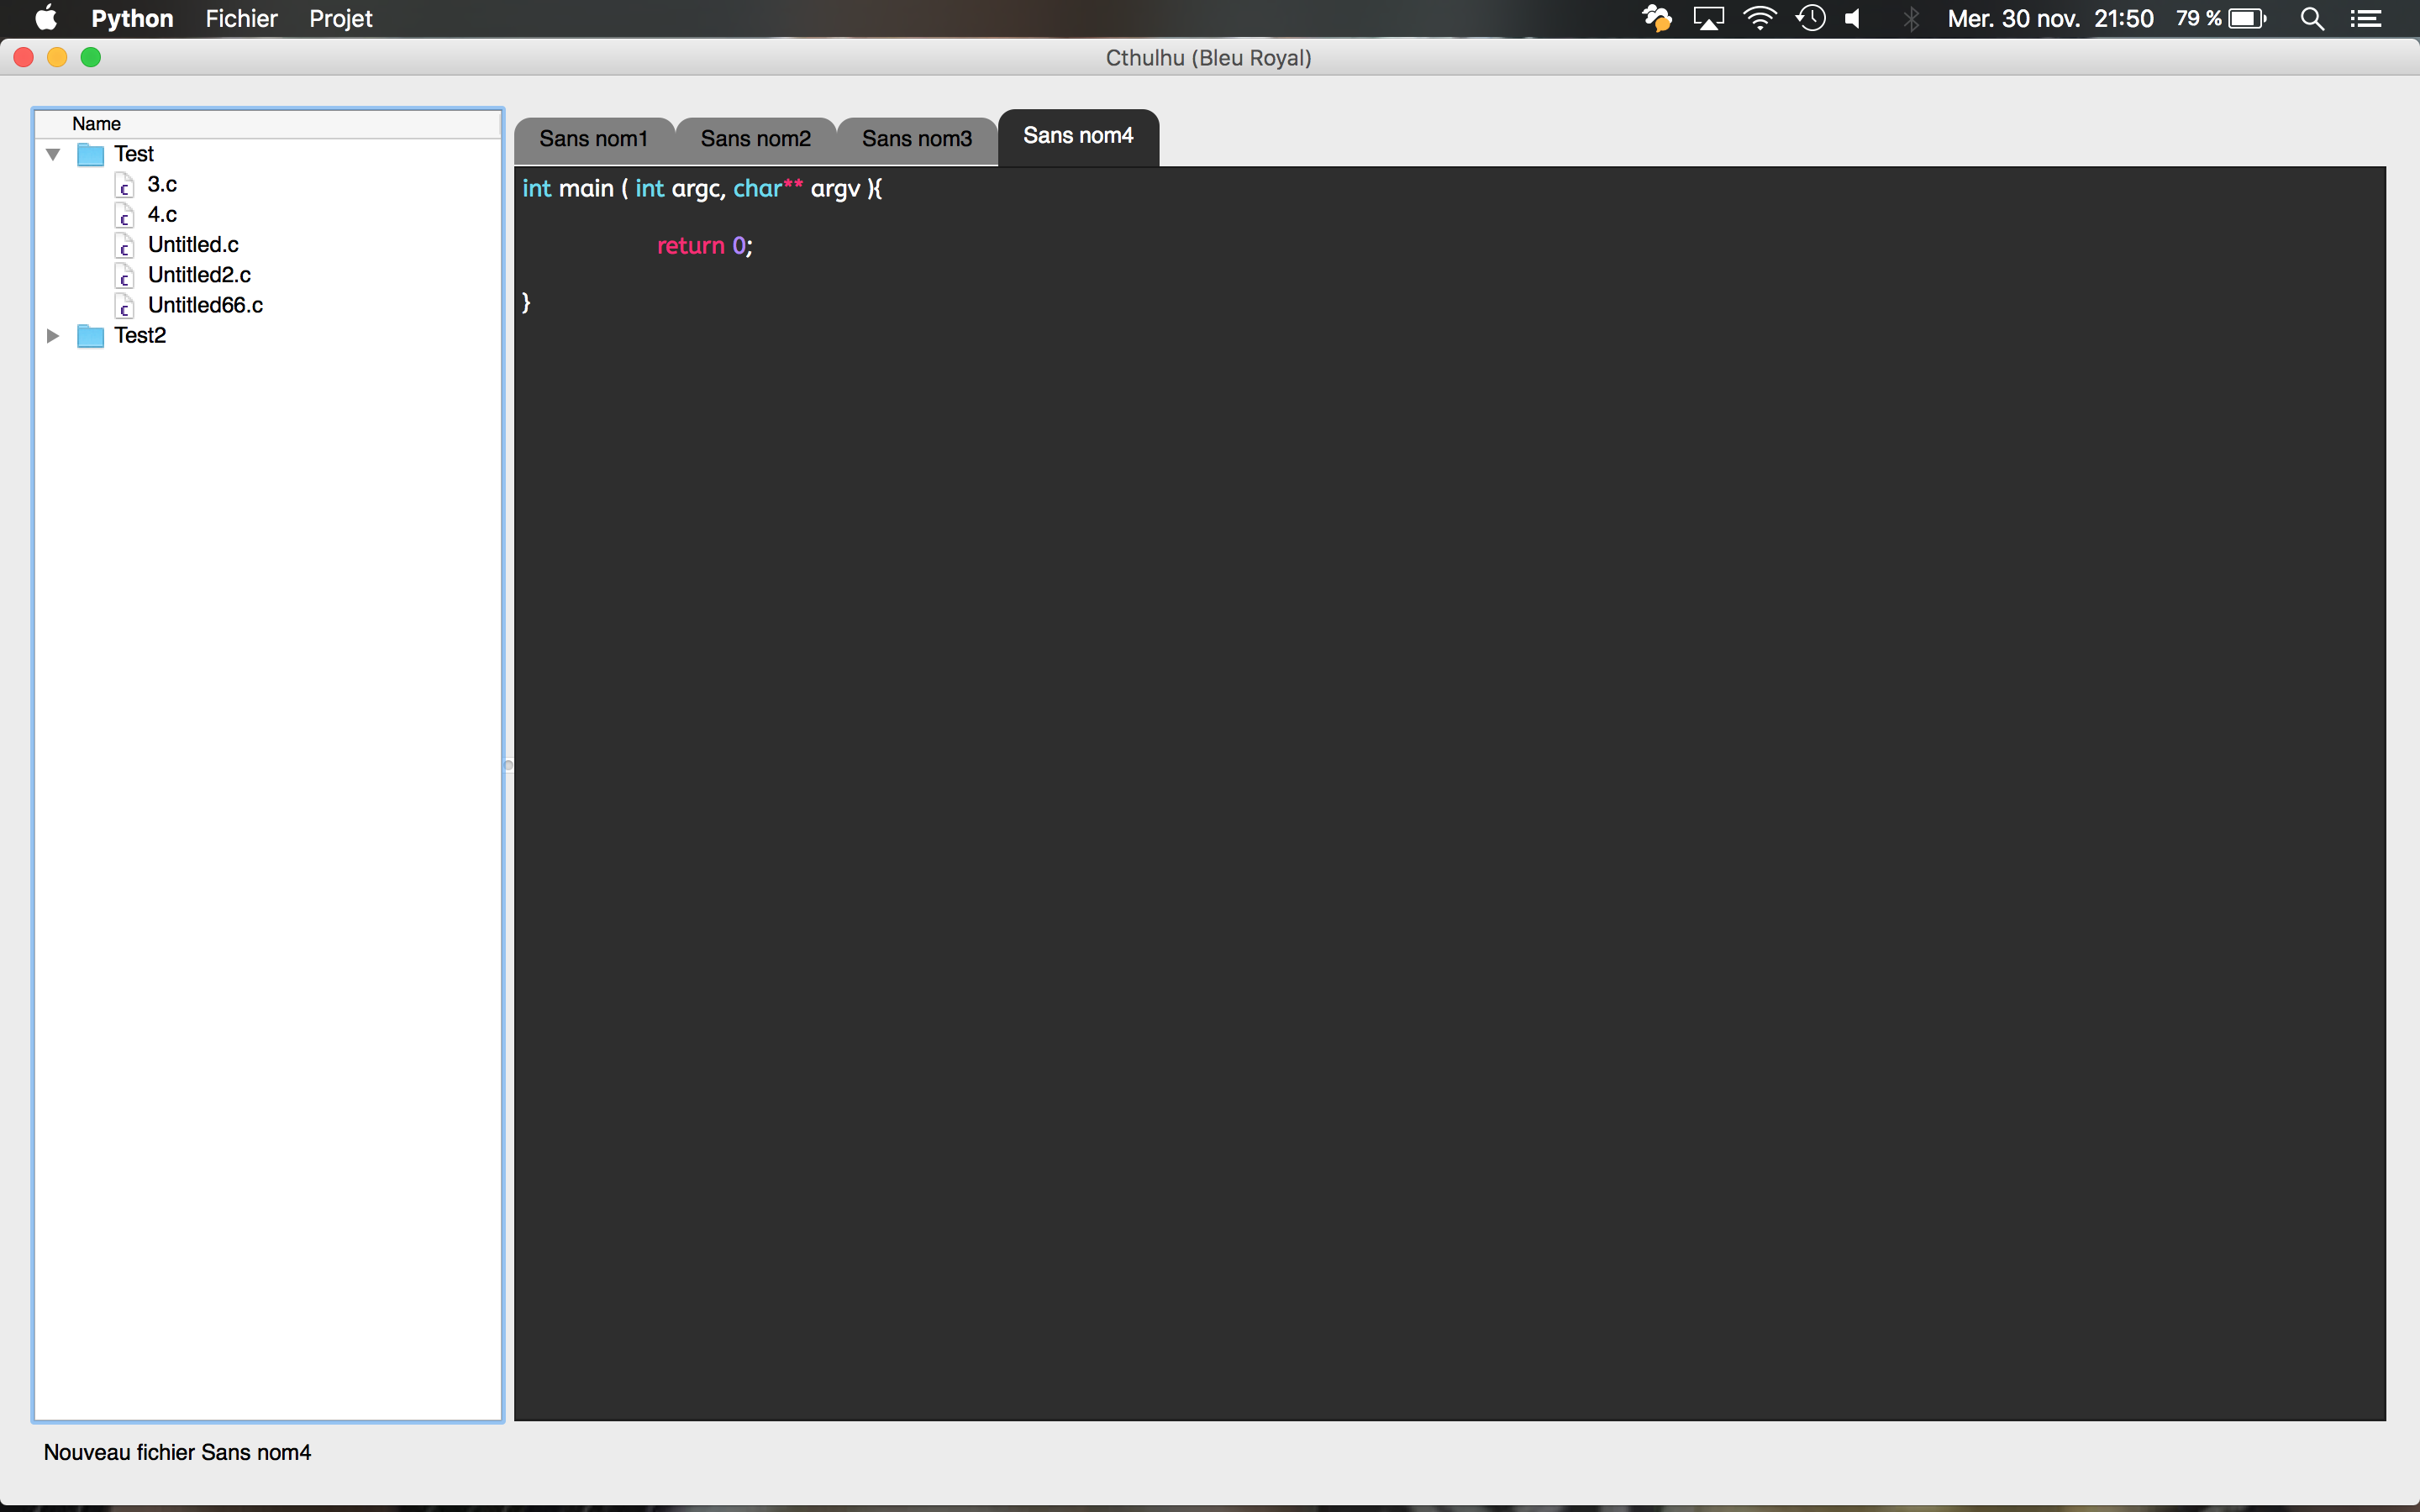
\includegraphics[scale=0.3]{images/ide_v1.png}
	
	Nous colorions le contenu des documents à l'aide du logiciel Lex, en particulier les différents tokens (éléments du code) selon leur fonction. Et nous analysions les documents pour détecter des erreurs de syntaxe à l'aide du logiciel Yacc. Nous utilisons pour cela une grammaire.
	
	\subsection{Grammaire pour Lex et Yacc}
	
		À l'aide du module PLY (Python Lex and Yacc), nous définissons une liste de tokens afin de déterminer tous les mots clefs du langage.
		
		\begin{figure}[!h]
			\begin{center}
				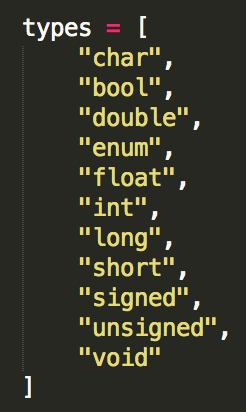
\includegraphics[scale=0.6]{images/tokens}
				\caption{Exemple de liste de tokens pour les déclarations de type en C.}
			\end{center}
		\end{figure}
		
		\newpage
		
		Nous avons aussi des fonctions à définir, pour Yacc afin de définir la syntaxe à suivre pour le langage (ici le langage C).
		Pour donner un exemple, sur les expressions de multiplication, nous indiquons qu'une multiplication peut prendre plusieurs formes.
		
		\begin{figure}[!h]
			\begin{center}
				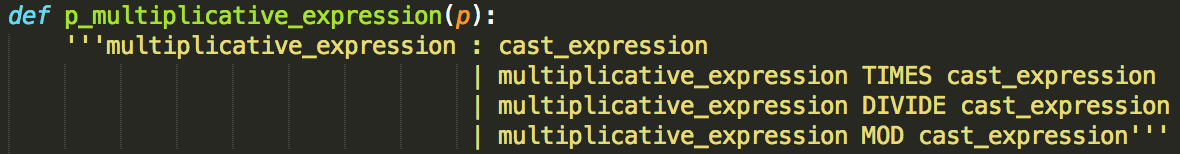
\includegraphics[scale=0.7]{images/yacc1}
				\caption{Différentes formes d'expressions de multiplication.}
			\end{center}
		\end{figure}
		
		Soit une "cast\_expression", soit une expression multiplicative multipliée par une "cast\_expression", soit une expression multiplicative divisée par une "cast\_expression" ou soit expression multiplicative modulo une "cast\_expression".
		
		\begin{figure}[!h]
			\begin{center}
				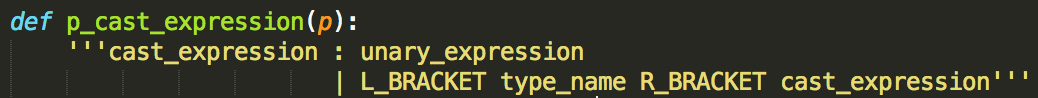
\includegraphics[scale=0.7]{images/yacc2}
				\caption{Une "cast\_expression"}
			\end{center}
		\end{figure}
		
		Une "cast\_expression" étant définie par une expression unitaire ou bien un "type\_name" entre parenthèses suivi d'une "cast\_expression". Où un "type\_name" est une autre fonction définissant ce que c'est.
		
		\begin{figure}[!h]
			\begin{center}
				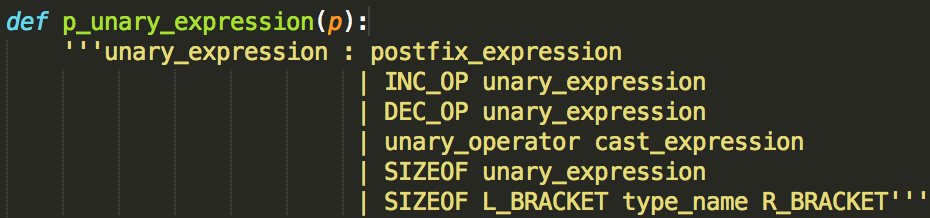
\includegraphics[scale=0.7]{images/yacc3}
				\caption{Une expression unitaire}
			\end{center}
		\end{figure}
		
		On décrit ci-dessus toutes les formes possibles d'expressions unitaires. C'est donc ainsi de suite et en remonttant toutes les clauses que l'on définit les règles syntaxiques du langage.
		
	\subsection{Pour ce semestre}
	
		Nous avons beaucoup travaillé pour rajouter de nombreuses fonctionnalités à notre éditeur afin qu'il soit complet et qu'il ressemble à des éditeurs déjà existant au niveau du contenu.\\
		
		Voici donc la liste de ce qui a été ajouté depuis les vacances de Noël :
		
		\begin{itemize}
			\item Différents thèmes et styles pour l'éditeur et ses éléments
			\item Traitement des projets
			\item Fichiers de configuration au format XML
			\item Intégration d'un compilateur
			\item Fonctionnalités diverses de recherche et d'édition de texte
			\item Inspecteur d'éléments
			\item Une autre barre de statut pour d'autres types d'informations
			\item Les numéros de lignes
			\item Fenêtre de paramétrage des raccourcis
			\item Ajout de cache afin d'optimiser l'ouverture de fichiers
			\item Grammaire arithmétique puis grammaire python
			\item Ajout de l'Anglais
			\item Quelques bonus \\
		\end{itemize}
		
		\textit{À noter que nous avions réalisé des rapports au fur et à mesure de l'avancement. Nous les reprennons ici donc en les ré-adaptant à l'aspect global évidemment. Mais il peut rester des images notamment sur la barre de menu où les fonctionnalités ne sont plus placées au même endroit. Par exemple, le menu apparence est maintenant placé dans Fichier/Paramètres.}
		
		
\section{Les thèmes et les styles}
	
	Afin de pouvoir rendre plus personnalisable l'application, nous avons choisi de permettre la personnalisation du thème global.
	Voici quelques exemples de thèmes : 
	
	
		\begin{figure}[h!]
			\begin{center}
				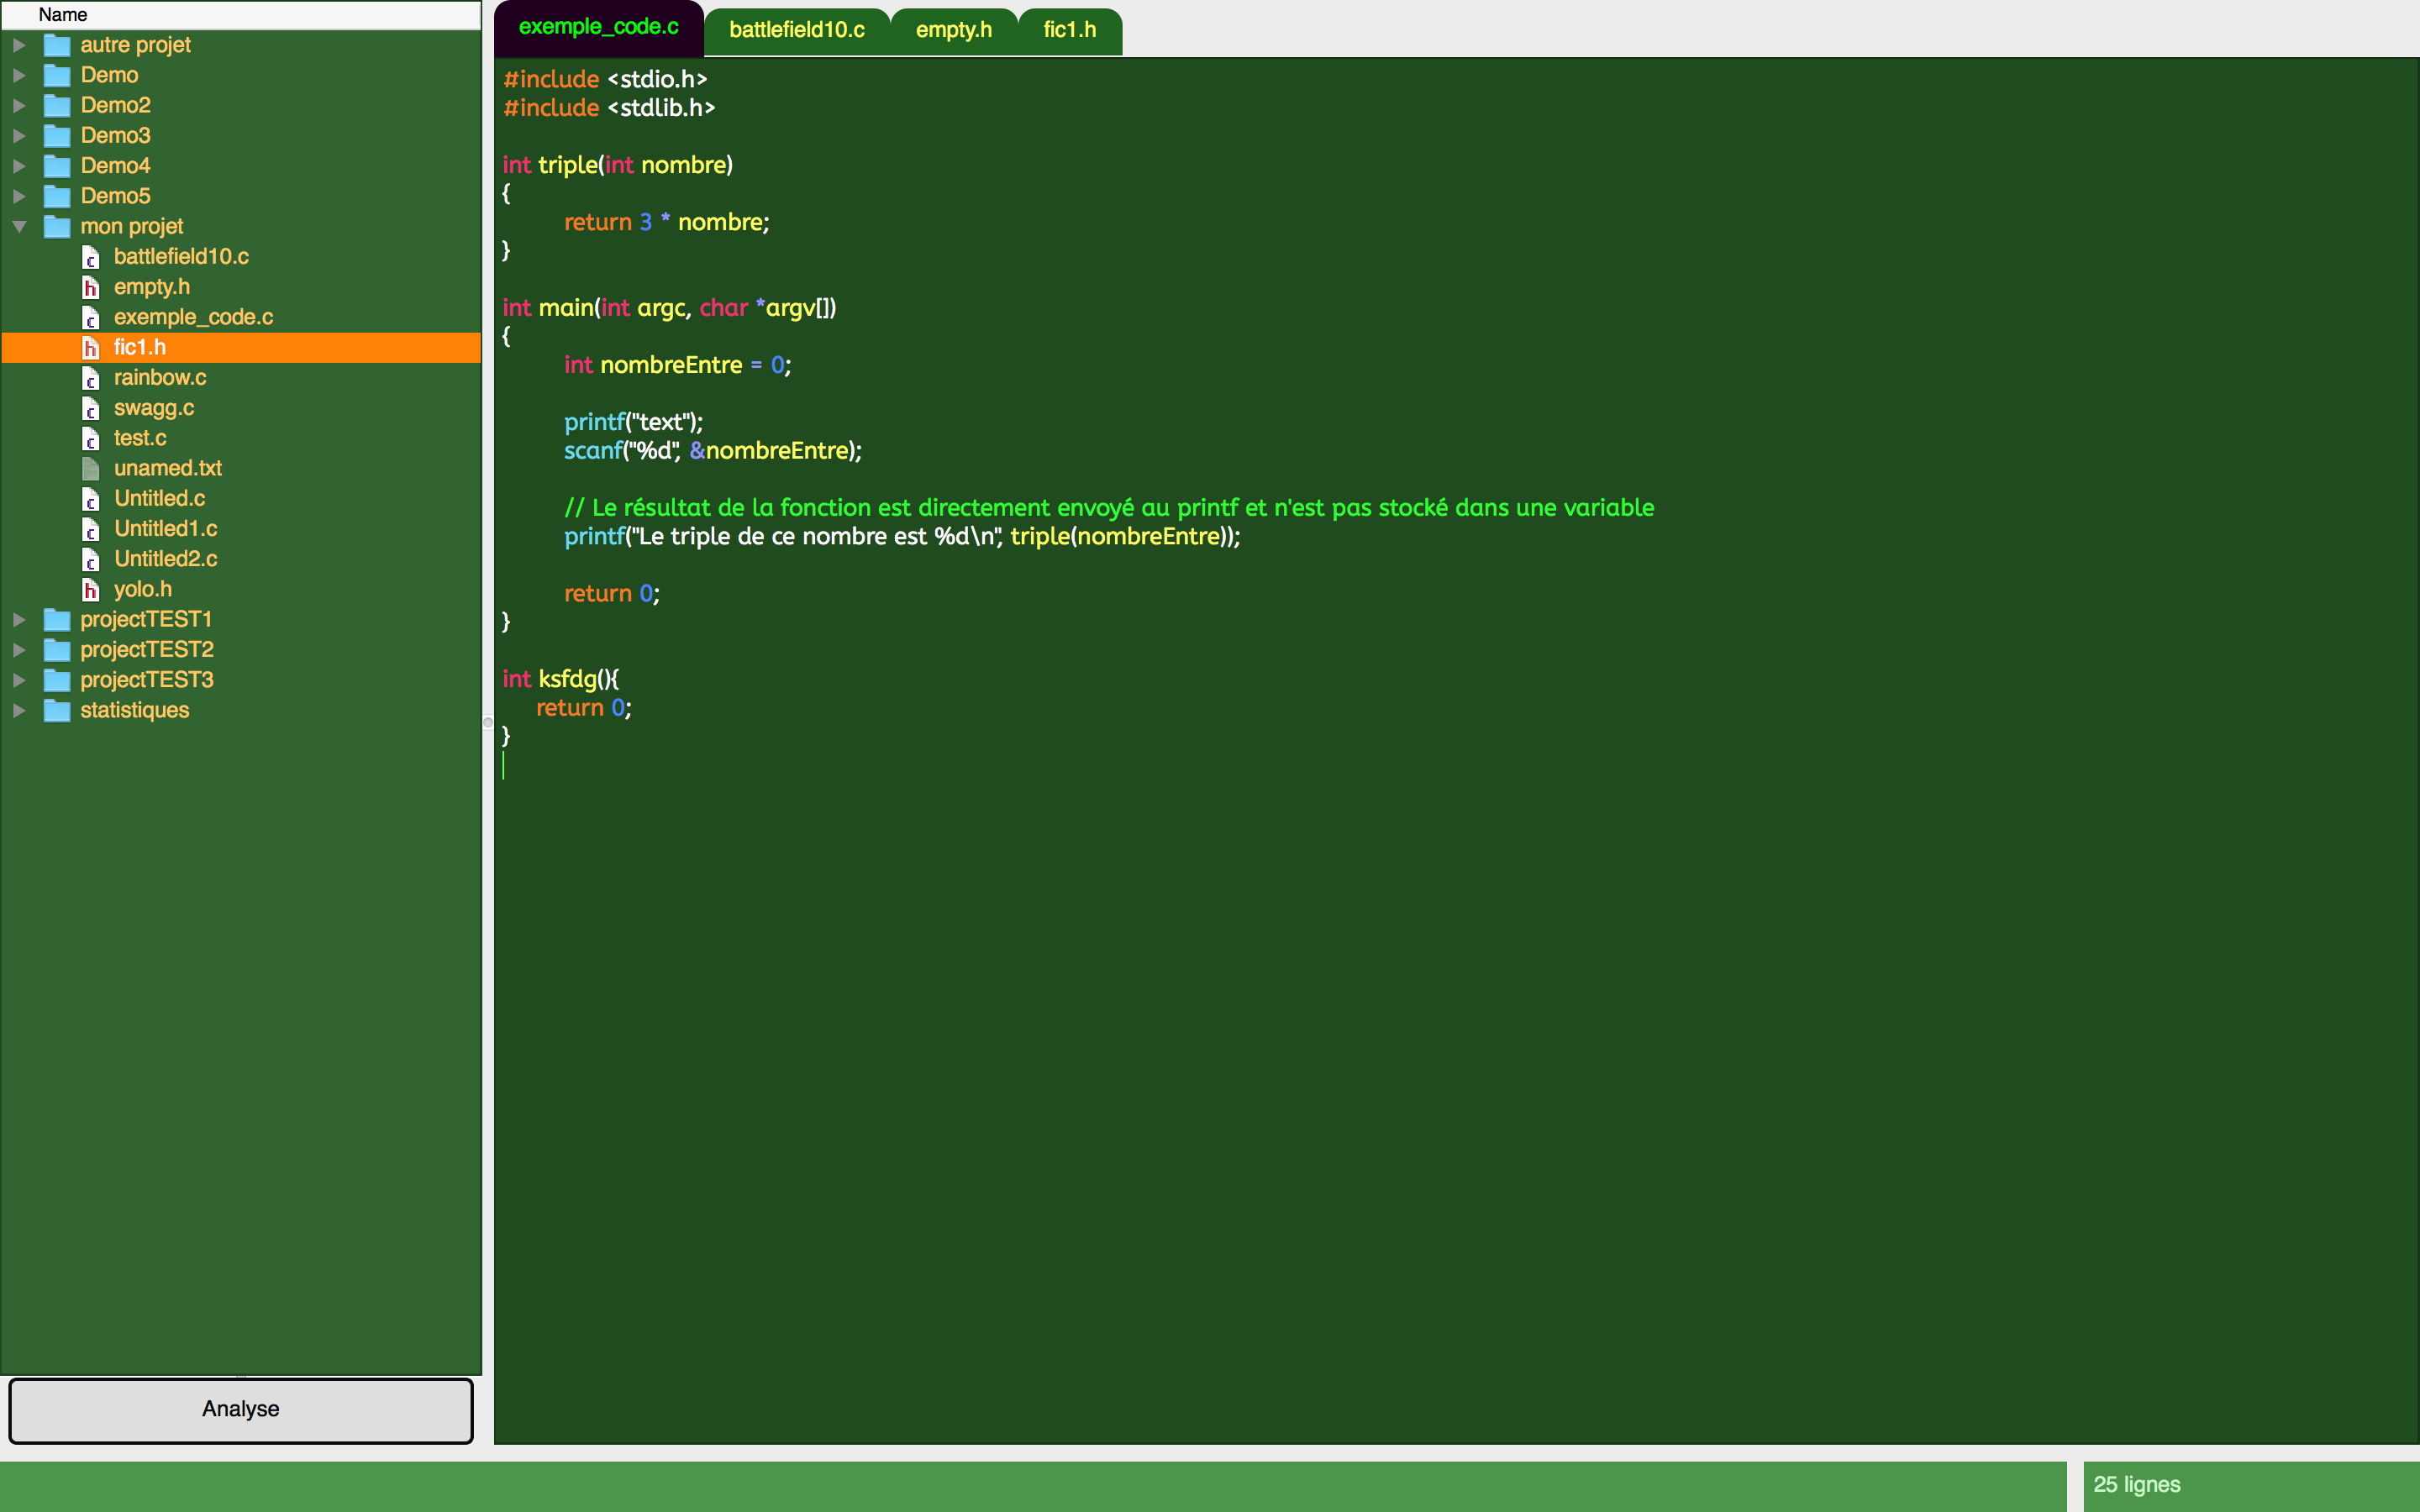
\includegraphics[scale=0.2]{images/imgs_themes/theme_forest}
				\caption{Thème Forêt}
			\end{center}
		\end{figure}
		
		\begin{figure}[h!]
			\begin{center}
				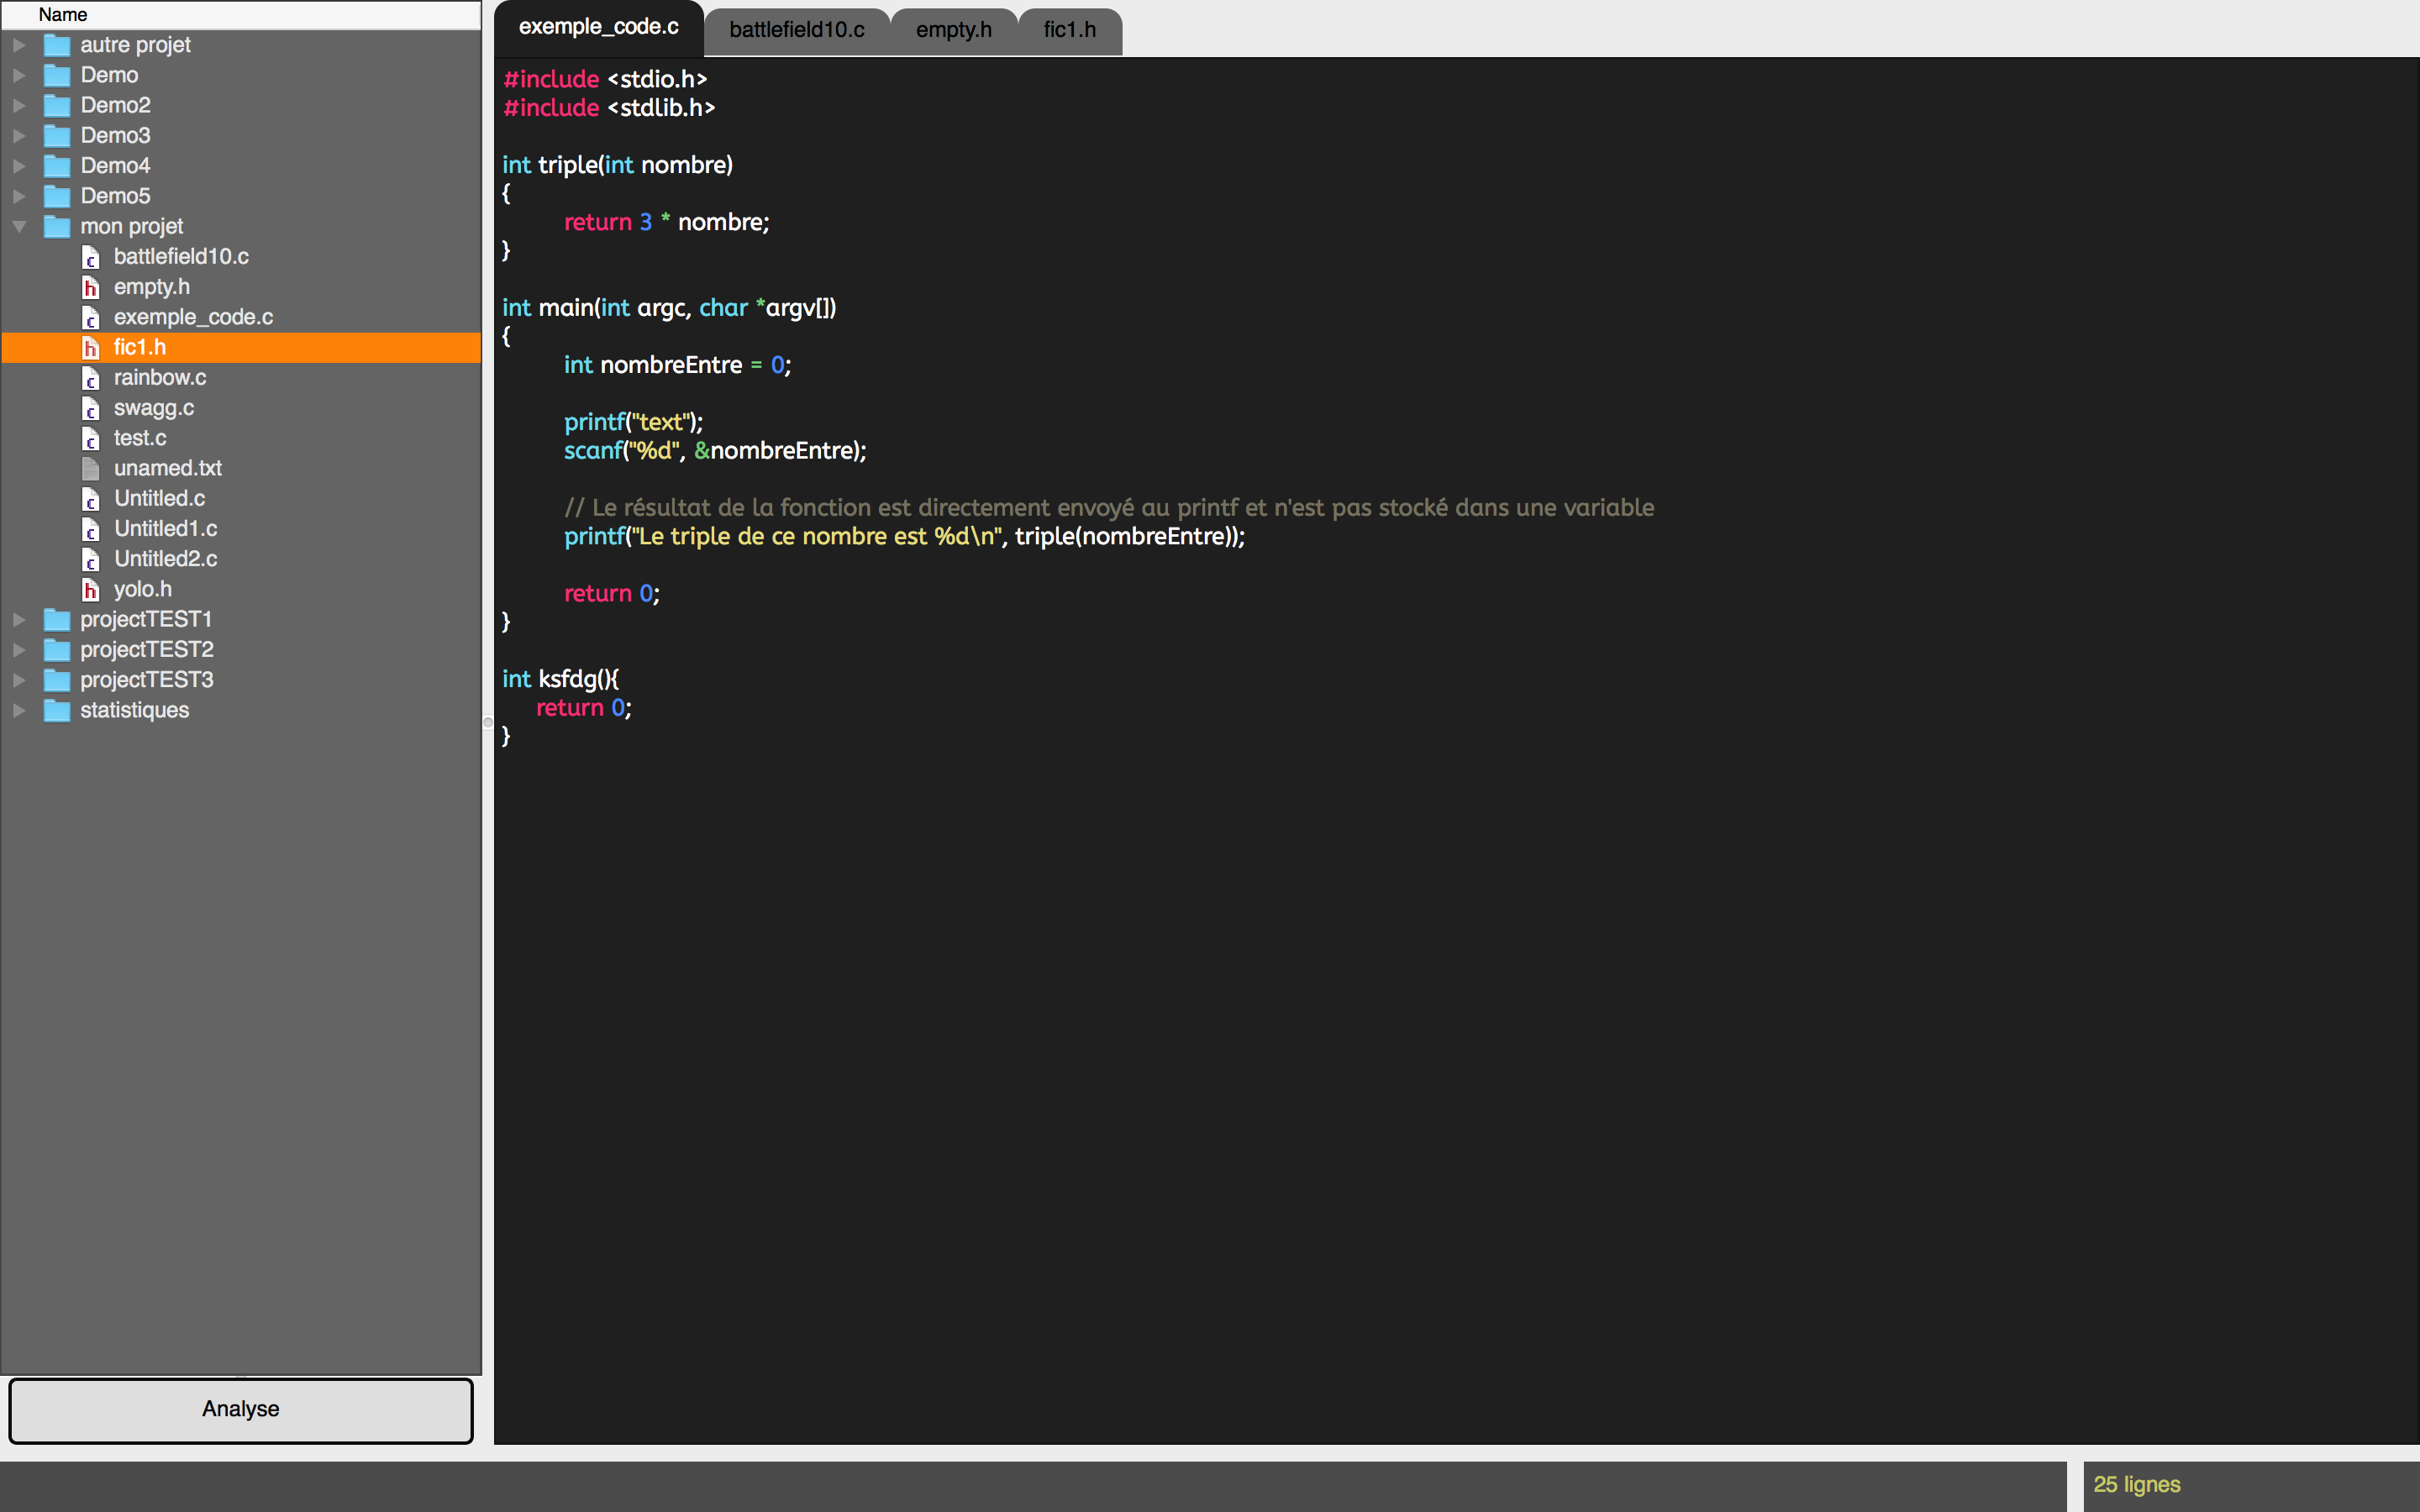
\includegraphics[scale=0.2]{images/imgs_themes/theme_basic}
				\caption{Thème de base}
			\end{center}
		\end{figure}
		
		\begin{figure}[h!]
			\begin{center}
				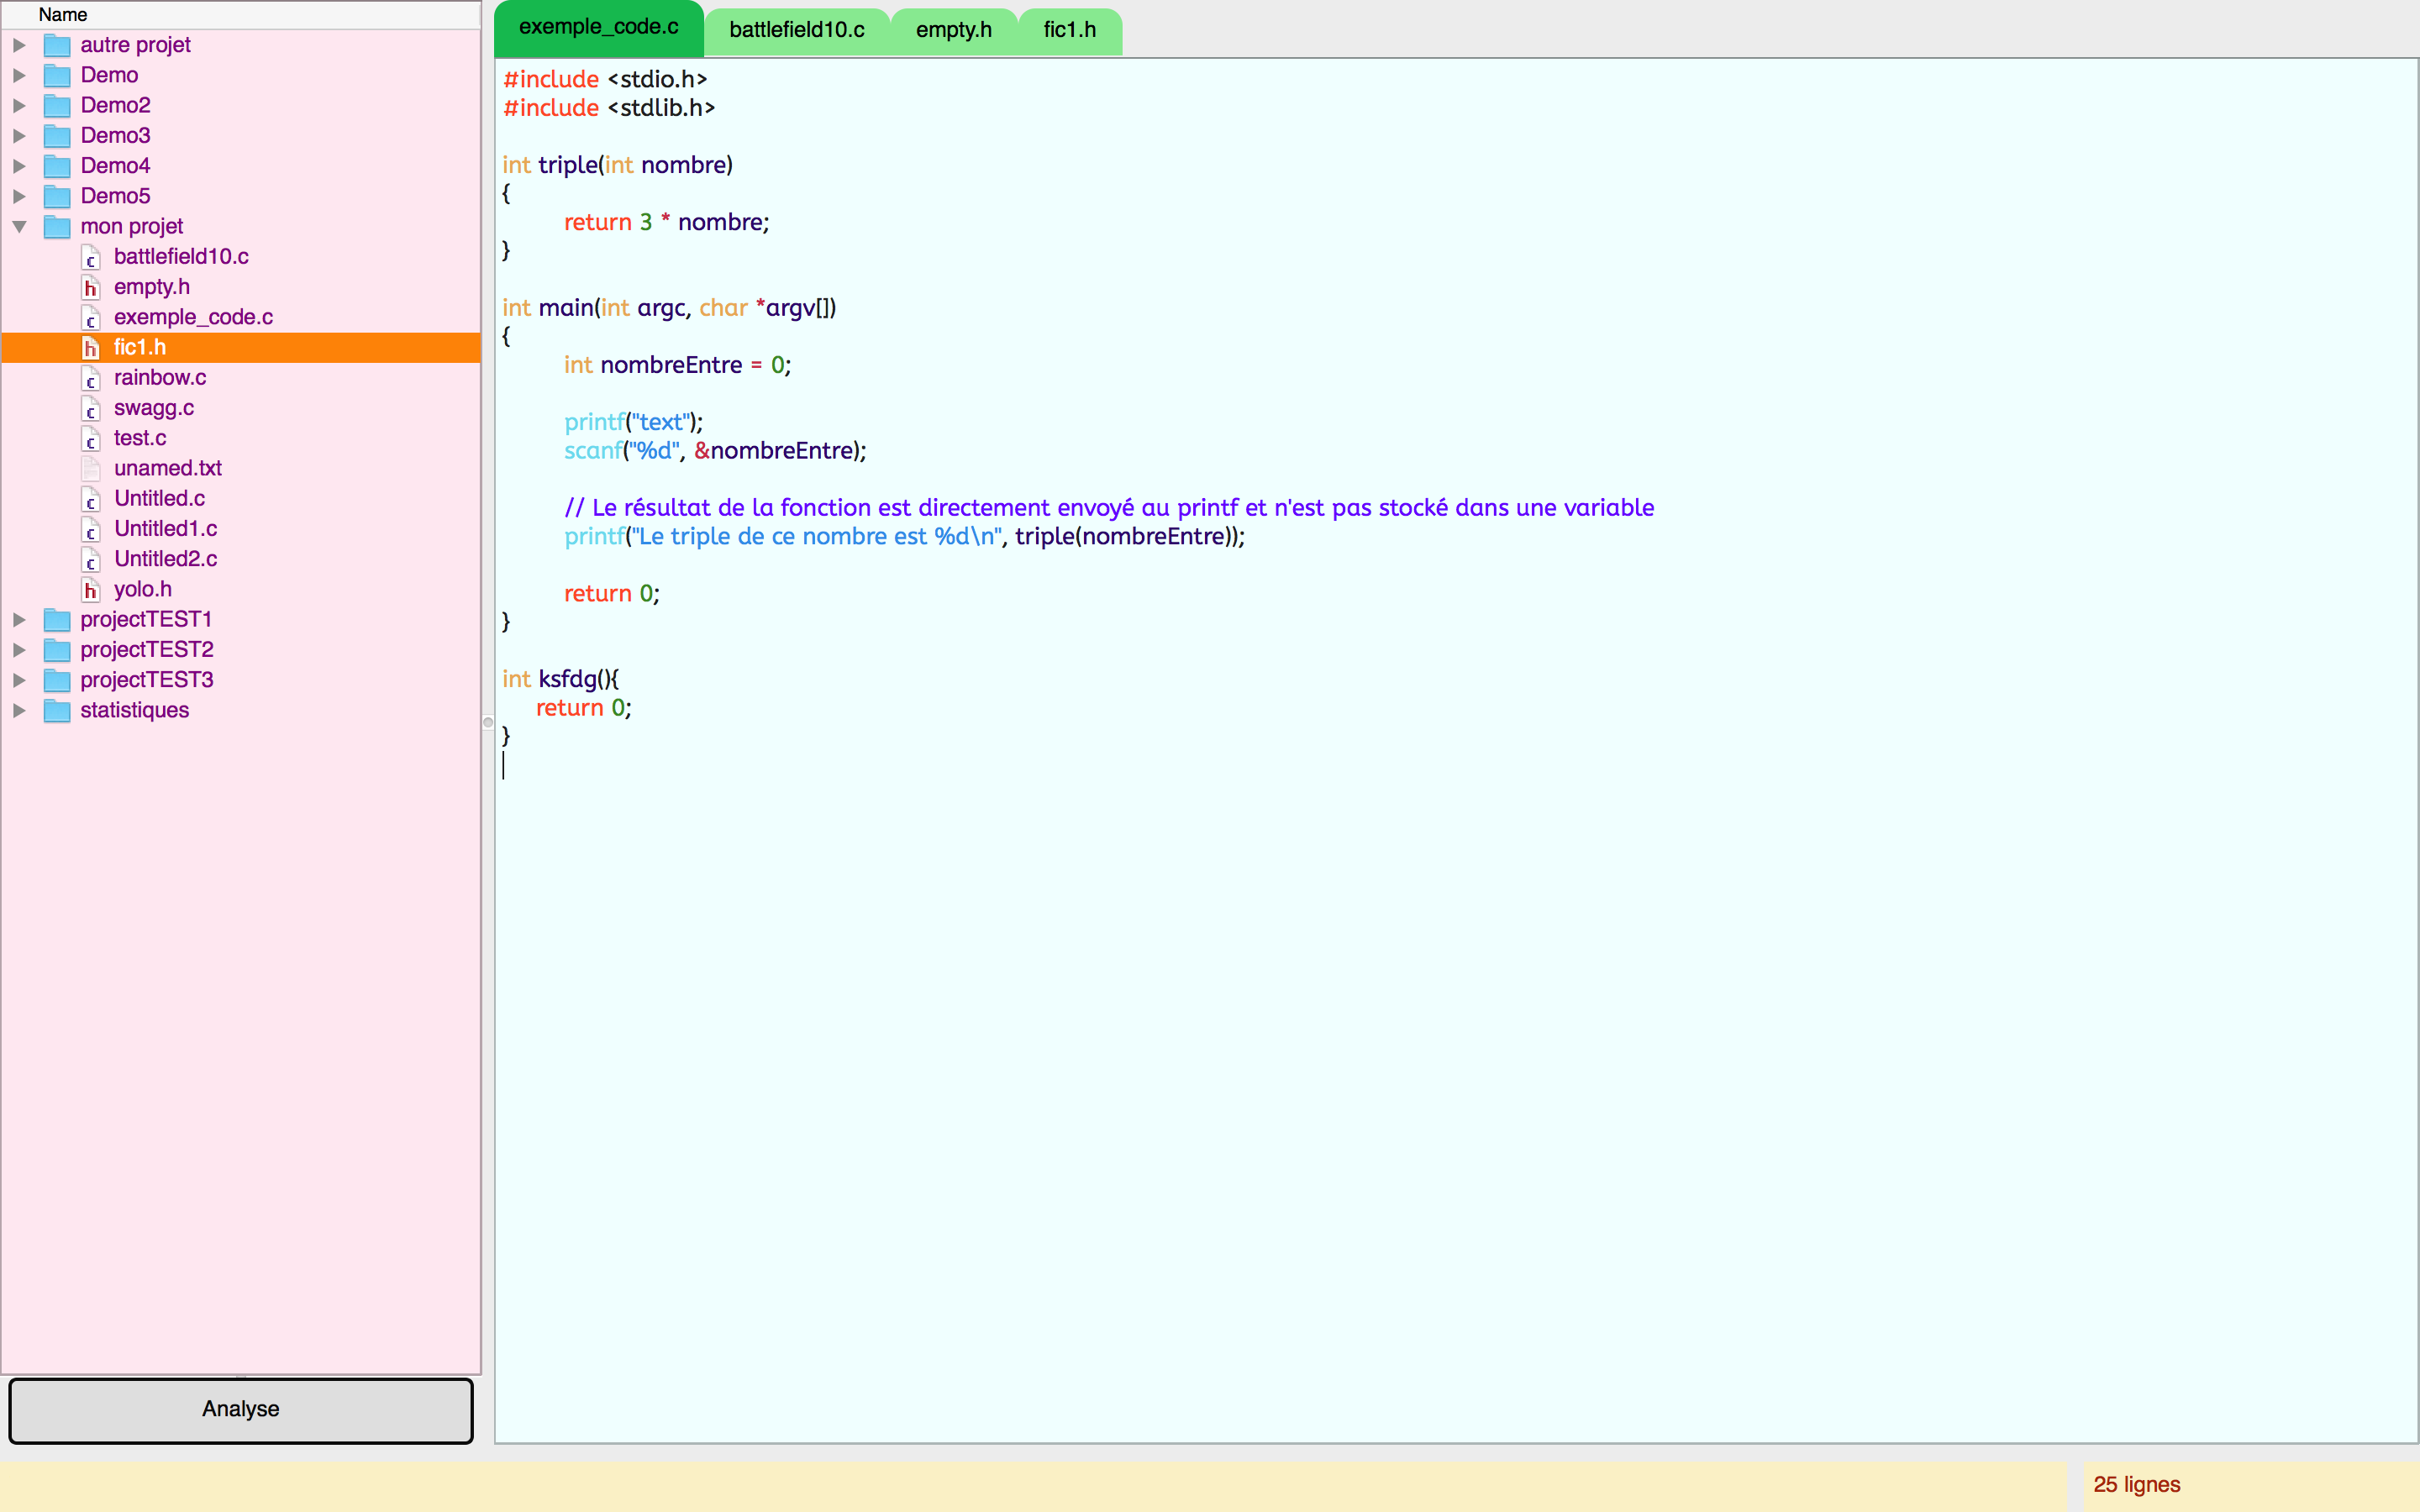
\includegraphics[scale=0.2]{images/imgs_themes/theme_pastel}
				\caption{Thème Pastel}
			\end{center}
		\end{figure}
		
		\newpage
		\subsection{Changer de thème}
		
			Le changement de thème est très simple. Il suffit de se rendre dans le menu "Fichier/Paramètres" puis de choisir son thème parmi ceux proposés dans les catégories clairs et sombres.
	
			\begin{figure}[h!]
				\begin{center}
					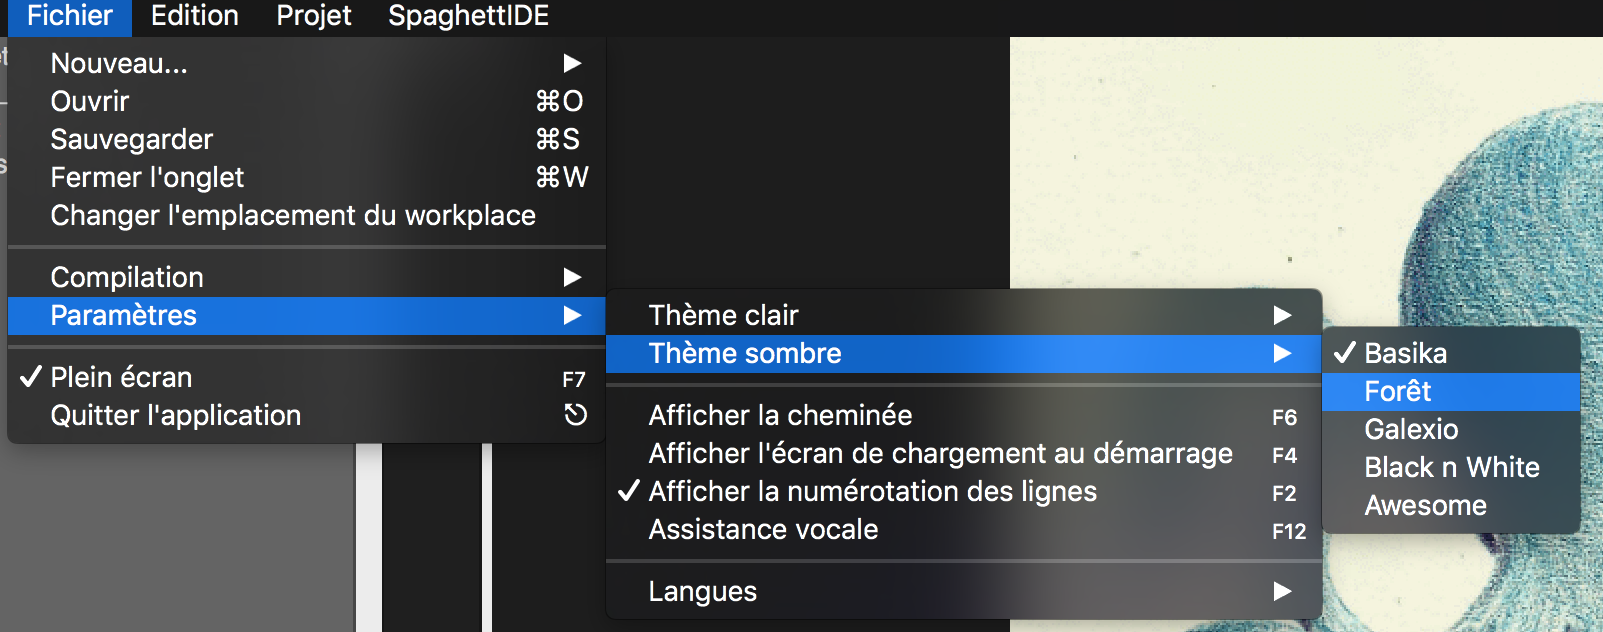
\includegraphics[scale=0.5]{images/imgs_themes/choix_theme}
					\caption{Choix de son thème}
				\end{center}
			\end{figure}
			
			Lorsqu'on sélectionne son thème il est immédiatement changé, il n'y a pas besoin de relancer l'application. De plus, une petite icone apparaît à côté du thème que vous avez choisi dans la barre de menu.\\
			
			Le thème sélectionné est alors écrit de le fichier conf.xml qui est situé à la racine du projet. Ainsi, lorsque vous relancerez l'IDE, le dernier thème que vous avez utilisé sera rechargé.
			
		\subsection{Gestion des thèmes}
		
			Les thèmes sont regroupés dans des répertoires distincts, le tout dans le répertoire "theme" situé à la racine du projet. 
			\begin{figure}[h!]
				\begin{center}
					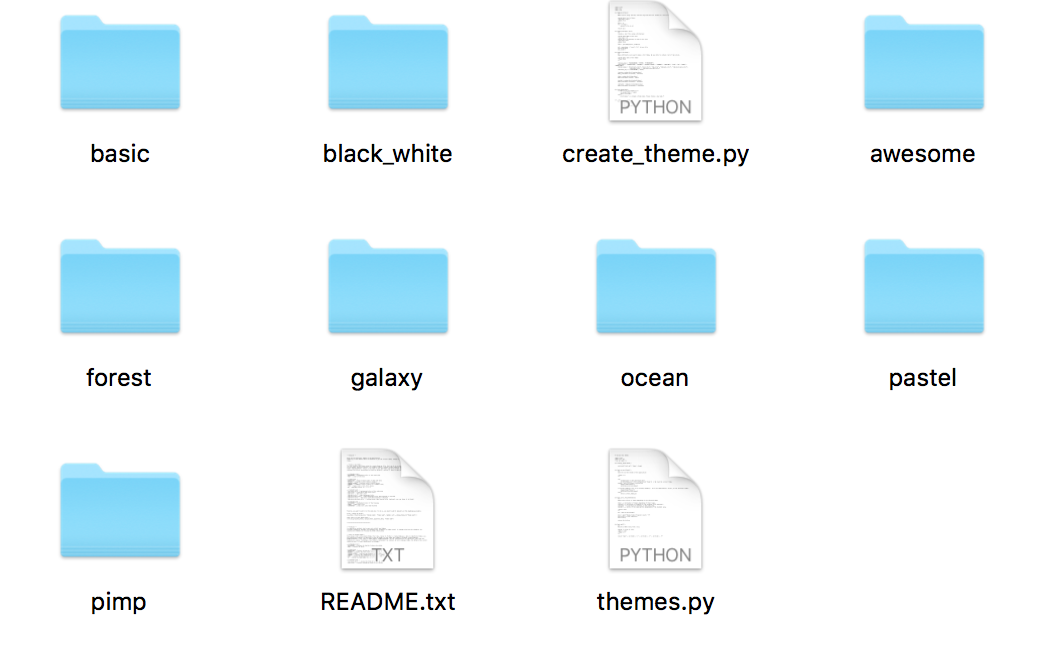
\includegraphics[scale=0.7]{images/imgs_themes/themes}
					\caption{Contenu du répertoire "theme"}
				\end{center}
			\end{figure}
			
			Chaque répertoire de thème regroupe les fichiers en format .json qui contiennent les couleurs en RGB de chaque élément de l'interface graphique.
			
			\begin{figure}[h!]
				\begin{center}
					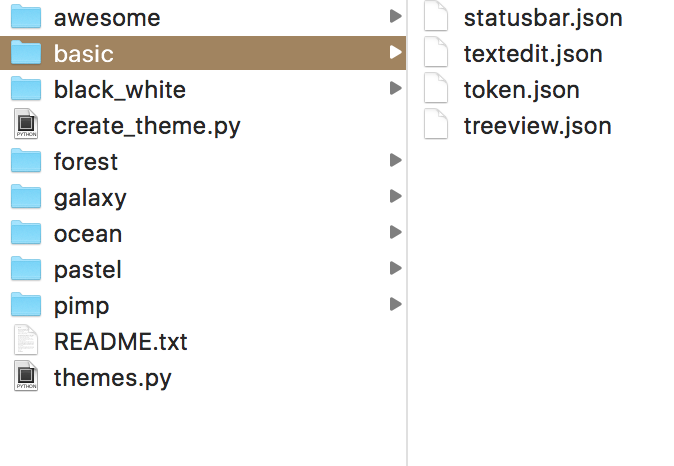
\includegraphics[scale=0.7]{images/imgs_themes/basic_json}
					\caption{Contenu du répertoire "basic" (le contenu est semblable pour tous les thèmes)}
				\end{center}
			\end{figure}
			\begin{figure}[h!]
				\begin{center}
					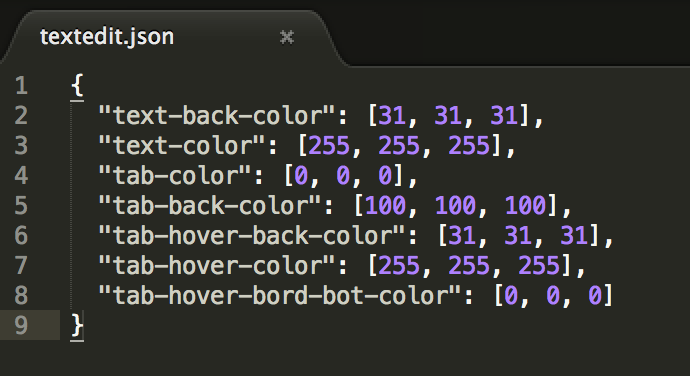
\includegraphics[scale=0.7]{images/imgs_themes/exemple_json}
					\caption{Exemple de fichier .json pour les thèmes.}
				\end{center}
			\end{figure}
			
			Le module theme.py nous permet de récupérer le thème sauvegardé (dans le fichier conf.xml) lors du chargement de l'application notament. Ici sont également contenues les méthodes permettant à l'interface d'aller chercher les couleurs qu'elle doit appliquer aux différents éléments.\\
			
			Au niveau technique, nous utilisons la méthode .setStyleSheet() de QT qui peut s'appliquer à la majorité des widgets (tous dans notre cas) et qui nous permet donc de spécifier et de modifier les couleusr de fond ainsi que de police des widgets en fonction du thème choisi.
			
		\subsection{Création de thèmes}
		
			Vous pouvez utiliser les thèmes pré-définis, qui ont été pour la plupart validés et certifiés par la totalité du groupe comme étant jolis, mais vous pouvez aussi créer vos propres thèmes.\\
			
			Le script "createtheme.py" vous permet cela, et la démarche à suivre est expliquée dans le fichier README.txt.\\
			
			Pour résumer, on lance le fichier createtheme.py via un terminal en spécifiant le nom du thème. Tapez par exemple :
			"python3 createtheme.py monNouveauTheme" et cela créera un répertoire "monNouveauTheme" qui contiendra les fichiers nécessaires à la gestion de votre thème. Ouvrez ensuite les fichiers .json et définissez vos propres couleurs (par défaut tout est noir).\\
			
			Une fois cela fait, vous devrez ajouter deux lignes dans le module menu.py pour que votre thème apparaisse dans la séléction.

			\begin{figure}[h!]
				\begin{center}
					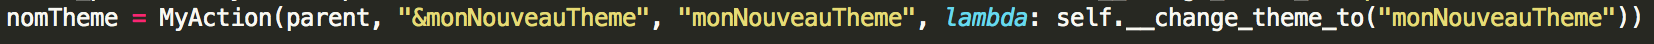
\includegraphics[scale=0.5]{images/imgs_themes/add2}
					\caption{Ici nomTheme est le nom de la variable pour le thème, et monNouveauTheme le nom que vous avez donné à votre thème}
				\end{center}
			\end{figure}
			\begin{figure}[h!]
				\begin{center}
					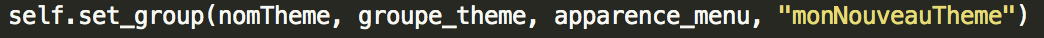
\includegraphics[scale=0.7]{images/imgs_themes/add1}
					\caption{Ici nomTheme est le nom de la variable pour le thème, et groupetheme le groupe (clair ou sombre) auquel appartient votre thème}
				\end{center}
			\end{figure}
			
			Votre thème apparaît maintenant dans la barre de menu et il est sélectionnable !
					
		\subsection{Style externe}
	
		Dans le répertoire "gui" qui contient tout ce qui est relatif à l'interface graphique, il y a un répertoire "style" qui regroupe des éléments auxquels on applique également des feuilles de styles (via la méthode setStyleSheet() des widgets dans QT; de même que pour les thèmes).
		
		\begin{figure}[h!]
			\begin{center}
				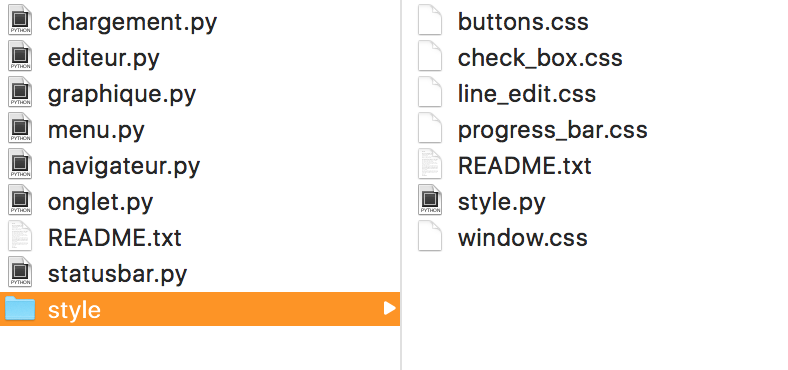
\includegraphics[scale=0.5]{images/imgs_themes/style}
				\caption{Contenu du répertoire style}
			\end{center}
		\end{figure}
		\newpage
				
		Chaque document .css contient le style relatif à des éléments. Nous retrouvons ici le style appliqué :
		
		\begin{itemize}
			\item aux boites de dialogue
				\begin{figure}[h!]
					\begin{center}
						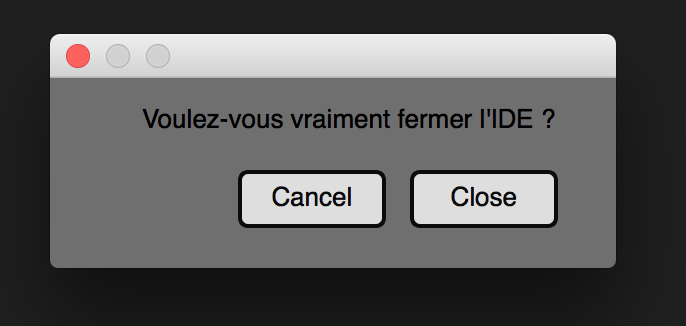
\includegraphics[scale=0.4]{images/imgs_themes/quit}
						\caption{ Exemple de la fermeture de l'IDE : une popup qui apparaît demandant la confirmation.}
					\end{center}
				\end{figure}
				
			\item aux boutons, à qui on inverse les couleurs lorsqu'on les survole
				\begin{figure}[h!]
					\begin{center}
						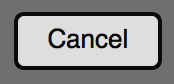
\includegraphics[scale=1]{images/imgs_themes/bout1}
						\caption{Style appliqué à un bouton normal.}
					\end{center}
				\end{figure}
				\begin{figure}[h!]
					\begin{center}
						
\includegraphics[scale=1]{images/imgs_themes/bout2}
						\caption{Le même bouton lorsqu'il est survolé par la souris.}
					\end{center}
				\end{figure}
				
			\item à la barre de progression
			\begin{figure}[h!]
					\begin{center}
						
\includegraphics[scale=0.7]{images/imgs_themes/progress2}
						\caption{La barre de statut (voir ci-dessous).}
					\end{center}
				\end{figure}
		\end{itemize}
		
\section{Informations sur le code}

	\subsection{Une autre barre de statut}
	
		Nous avons également travaillé à étoffer l'interface. Nous avons rajouté une seconde barre de statut (en bas à droite), servant à afficher des informations sur le code lui-même :
		
		\begin{figure}[h!]
			\begin{center}
				
\includegraphics[scale=1]{images/imgs_themes/nb_lignes}
				\caption{Le nombre de lignes du fichier courant}
			\end{center}
		\end{figure}
		\begin{figure}[h!]
			\begin{center}
				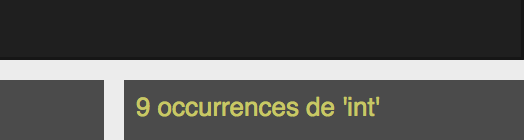
\includegraphics[scale=1]{images/imgs_themes/nb_occu}
				\caption{Le nombre d'occurences d'une recherche effectuée}
			\end{center}
		\end{figure}
		
		Nous utilisons de plus cet emplacement (en bas à droite) pour afficher une barre de statut qui sert à indiquer la progression lors du chargement de projet (Yacc lisant tous les fichiers afin de récupérer les différentes fonctions à travers les modules, cela peut prendre plusieurs secondes).
		\begin{figure}[h!]
			\begin{center}
				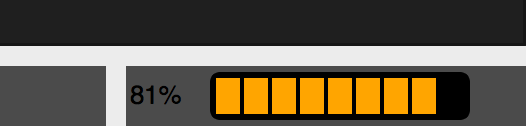
\includegraphics[scale=1]{images/imgs_themes/progress}
				\caption{Barre de progression lors du chargement d'un projet de l'utilisateur}
			\end{center}
		\end{figure}
		
		L'ouverture de projets est maintenant beaucoup plus rapide qu'au début du semestre, notament grâce à l'utilisation du cache. La barre de progression apparaît toujours, mais c'est souvent très rapide.
		
	\subsection{Numérotation des lignes}
	
	\subsubsection{Insertion dans l'interface graphique}

	L'objet que nous utilisons pour afficher et éditer le code est un QTextEdit de QT. Il ne possède pas de méthode pour afficher les numéros de lignes, et il n'y a pas d'autres alternatives à celui-ci pour faire cela non plus.
	
	Il nous fallait donc un autre élément, afin d'afficher les numéros de lignes qui serait placé sur le côté, nous avons choisi le côté droit.
	
		\begin{figure}[h!]
			\begin{center}
				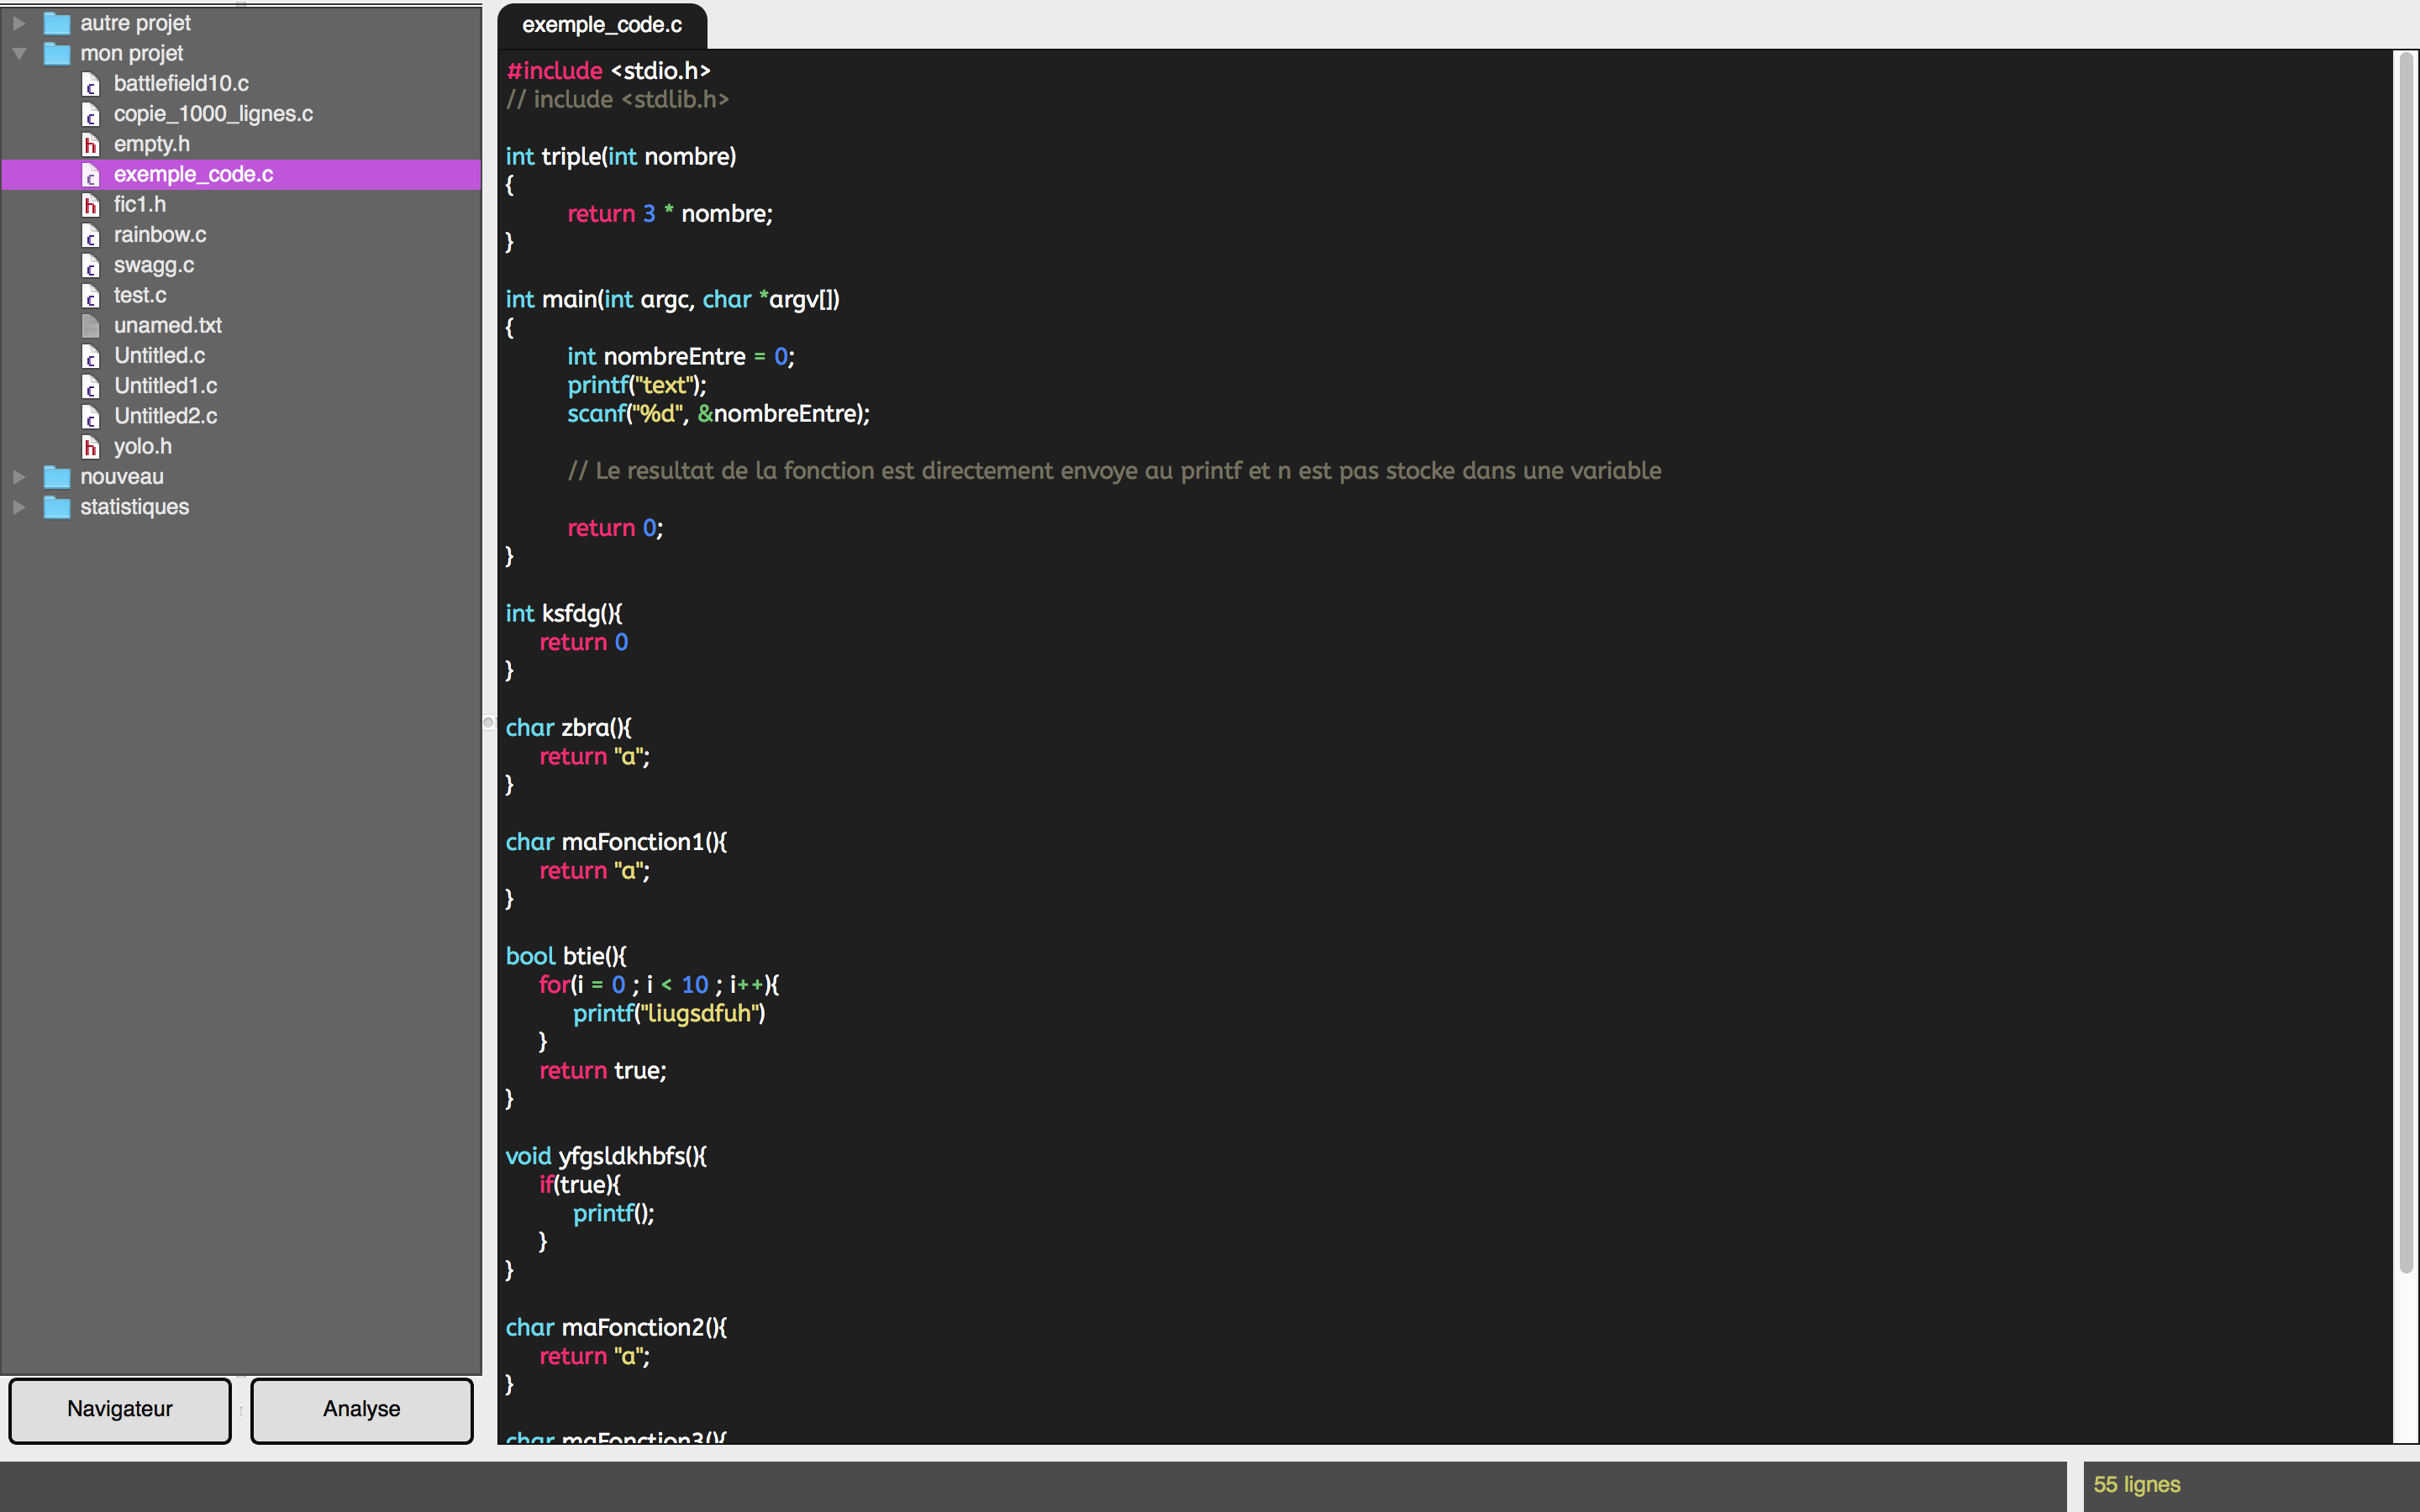
\includegraphics[scale=0.17]{images/imgs_lines/avant}
				\caption{Sans la barre de numérotation des lignes}
			\end{center}
		\end{figure}
		
		\begin{figure}[h!]
			\begin{center}
				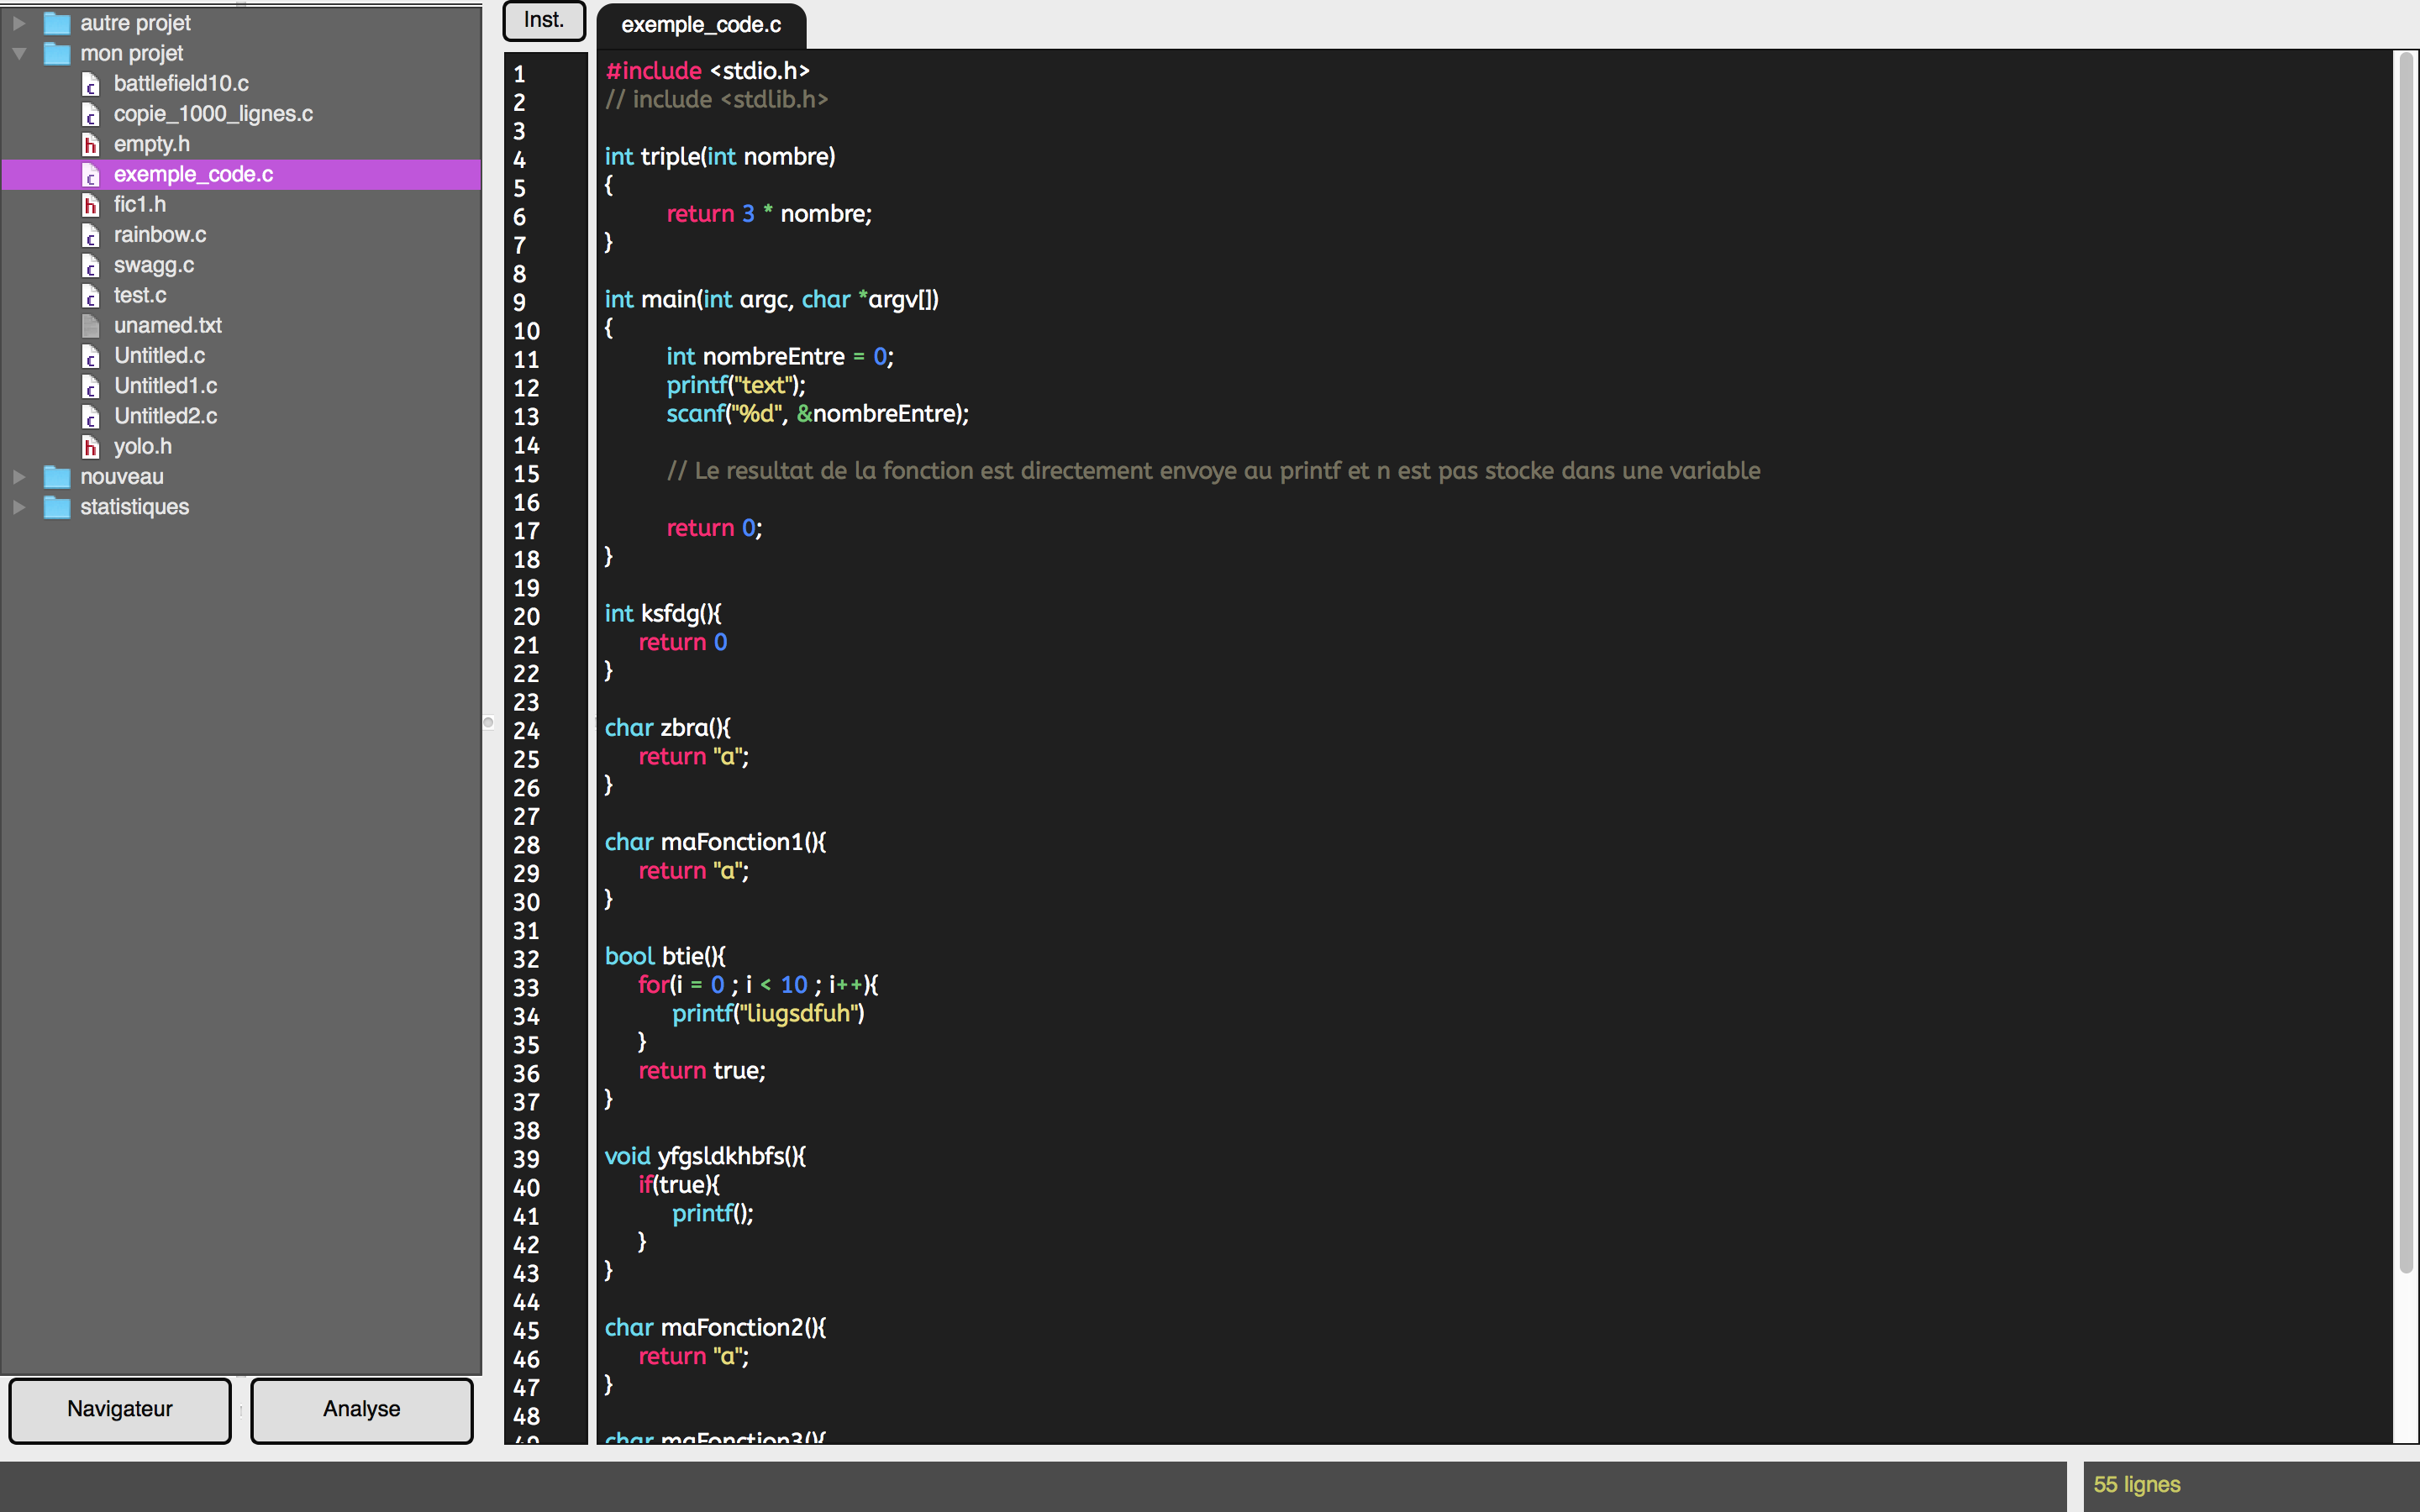
\includegraphics[scale=0.17]{images/imgs_lines/apres}
				\caption{Avec la barre de numérotation des lignes}
			\end{center}
		\end{figure}
		
		\newpage
		
	L'utilisateur peut choisir d'afficher ou non cette barre.
	
		\begin{figure}[h!]
			\begin{center}
				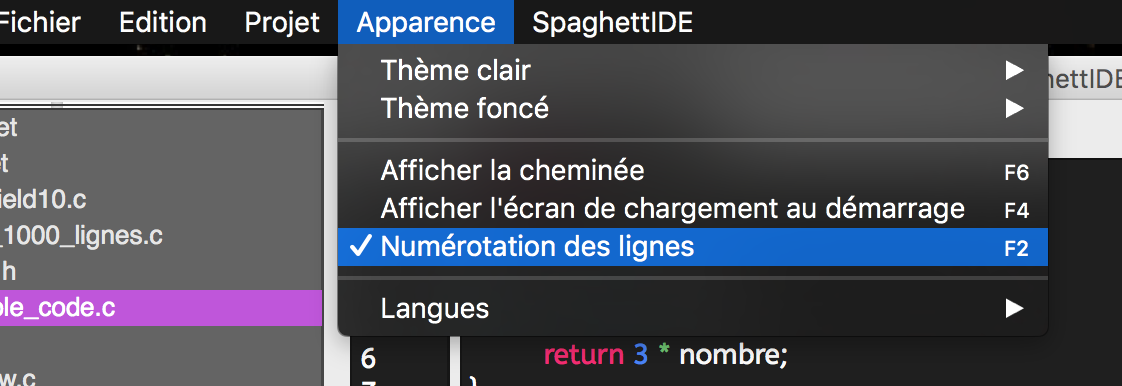
\includegraphics[scale=0.8]{images/imgs_lines/menu}
				\caption{Dans le menu apparence}
			\end{center}
		\end{figure}
		
	\subsubsection{Surcharger les méthodes originales}

	La difficulté n'était pas d'afficher une barre avec des numéros dedans, ni de récupérer le nombre de lignes, car nous avons une méthode pour cela. La difficulté était de syncroniser le défilement des deux éléments (widgets).\\
		
		Lorsque l'on fait un défilement avec la molette de souris ou le pad \textbf{uniquement}, la méthode appelée sur le QTextEdit est le "wheelEvent(e)" où "e" est l'évenement utilisé par QT pour effectuer le défilement.\\
		
		Le principe consiste à appeler la fonction d'origine ainsi que celle de l'autre objet avec le même argument "e" lorsque la méthode "wheelEvent()" est appelée.
		
		\newpage
		
		\begin{figure}[h!]
			\begin{center}
				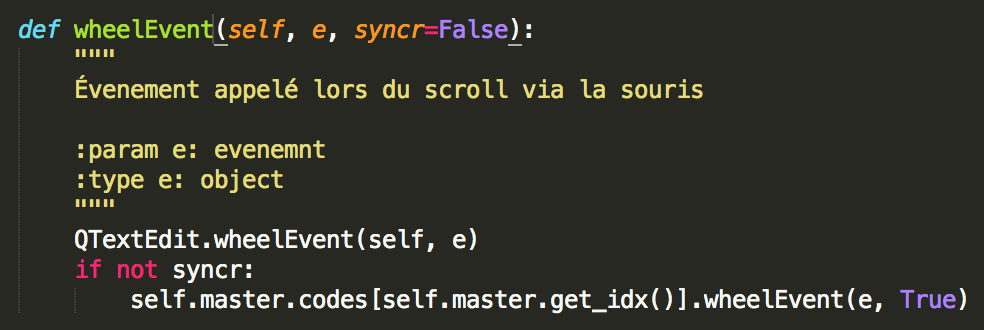
\includegraphics[scale=0.9]{images/imgs_lines/wheel_lines}
				\caption{Méthode de l'objet contenant la numérotation des lignes}
			\end{center}
		\end{figure}
		
		
		Ici, "self.master.codes" désigne la liste des onglets de codes ouverts, et "self.master.get\_idx()" retourne l'indice de l'onglet courant. On appelle donc la méthode "wheelEvent()" de l'onglet courant lorsque l'on fait défiler la liste de numérotation des lignes. L'argument booléen sert à dire qu'il ne faut pas rappeler la méthode "wheelEvent()" car sinon on rentrerait dans une boucle infinie.\\
		
		\begin{figure}[h!]
			\begin{center}
				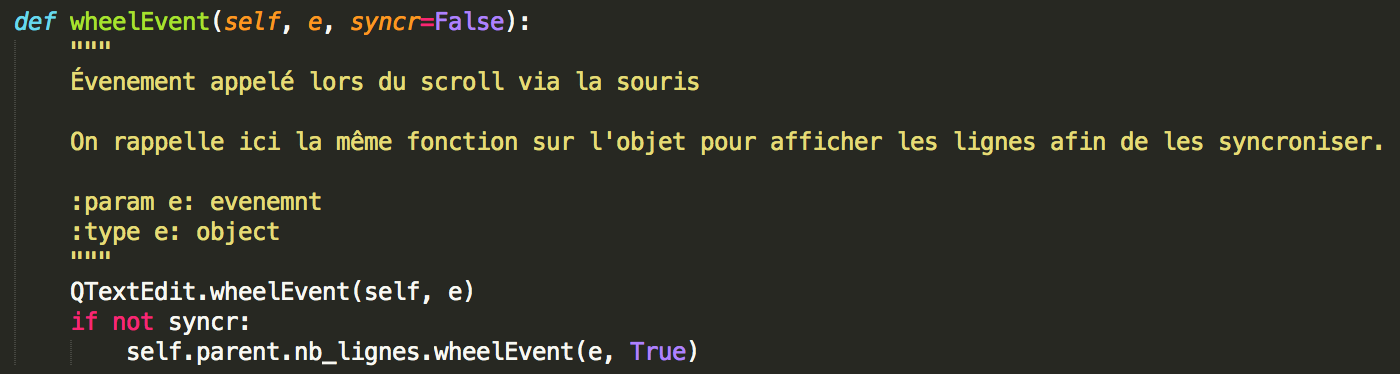
\includegraphics[scale=0.7]{images/imgs_lines/wheel_code}
				\caption{Méthode de l'objet contenant le code}
			\end{center}
		\end{figure}
		
		"self.parent.nb\_lignes" désigne l'objet contenant la numérotation des lignes, on y appelle donc la méthode "wheelEvent()" avec les même arguments. Et toujours l'argument empêchant la boucle infinie.\\
		
		Nous arrivons ainsi à syncroniser les deux éléments lors du défilement de l'un comme de l'autre avec la souris ou le pad.
		
		
\section{Recherche et édition du texte}

	\subsection{Selection de la ligne courante}

	Dans un premier temps, nous avons ajouté une fonction permettant de sélectionner la ligne où se trouve le curseur.
	Pour cela, nous récupérons l'objet QTextCursor de notre classe Editeur (héritant de QTextEdit) puis nous utilisons la méthode \textbf{select} de cet objet qui nous permet de sélectionner du texte dans notre Editeur, cette méthode prend en paramètre une méthode de selection, QTextCursor.LineUnderCursor dans notre cas. La ligne où se trouve notre cuseur va donc être selectionnée.
	Pour appliquer ces modifications, nous devons appliquer notre objet QTextCursor à notre Editeur, pour cela on utilise la méthode \textbf{setTextCursor} de l'objet Editeur et on lui passe en paramètre notre QTextCursor.  


	\begin{figure}[h!]
		\begin{center}
			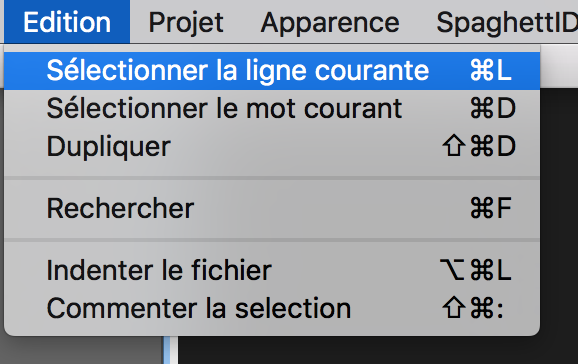
\includegraphics[scale=0.8]{images/imgs_edit/utilisation_selection_ligne}
			\caption{Action du menu permettant la sélection de la ligne courante}
		\end{center}
	\end{figure}

	\begin{figure}[h!]
		\begin{center}
			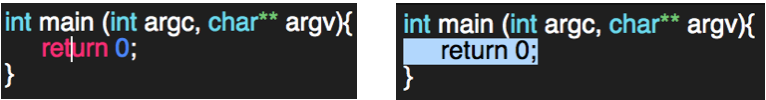
\includegraphics[scale=0.8]{images/imgs_edit/resultat_selection_ligne}
			\caption{Résultat de l'utilisation de la fonction sélection de la ligne courante}
		\end{center}
	\end{figure}

\subsection{Selection du mot courant}

	Pour l'ajout de la sélection du mot courant, la démarche est exactement la même que pour la sélection de la ligne courante, nous devons simplement changer la méthode de sélection, passant de QTextCursor.LineUnderCursor à QTextCursor.WordUnderCursor, afin de ne plus sélectionner la ligne mais le mot présent au niveau du curseur. 

	\begin{figure}[h!]
		\begin{center}
			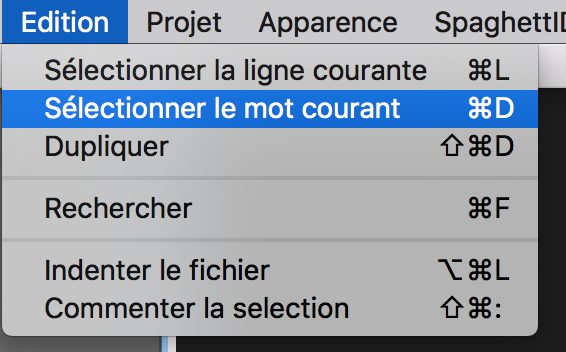
\includegraphics[scale=0.4]{images/imgs_edit/utilisation_selection_mot}
			\caption{Action du menu permettant la sélection du mot courant}
		\end{center}
	\end{figure}

	\begin{figure}[h!]
		\begin{center}
			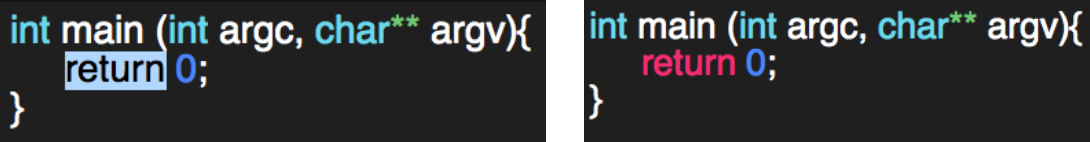
\includegraphics[scale=0.8]{images/imgs_edit/resultat_selection_mot}
			\caption{Résultat de l'utilisation de la fonction sélection du mot courant}
		\end{center}
	\end{figure}
	
	\newpage

\subsection{Duplication}

	Pour l'ajout de la duplication du texte, nous avons choisi de différencier deux cas, le premier où rien n'est selectionné et le second où du texte est déjà selectionné. Dans le premier cas toutes la ligne est dupliquée et dans le second seulement la partie selectionnée est dupliquée.

	Pour cela, nous récuppérons une nouvelle fois le QTextCursor de notre Editeur, puis pour savoir dans quel cas nous sommes on utilise la méthode selectedText de l'objet QTextCursor. Ainsi si aucun text n'est sélectionné nous sélectionnons la ligne courante de le même façon que précédement de plus on assigne la valeur  \textbf{\\n} à la variable \textbf{return\_} en effet si on duplique une ligne entière, on ajoute on retoure à la ligne entre la sélection d'origine et la partie dupliquée. Puis on ajoute le texte dans notre objet Editeur grâce à la méthode \textbf{inserText} avec en paramètre la sélection du QTextCursor (recuperrée grâce à la méthode \textbf{selectedText}) suivie de la variable \textbf{return\_} elle même suivie de la sélection du QTextCursor.

	\begin{figure}[h!]
		\begin{center}
			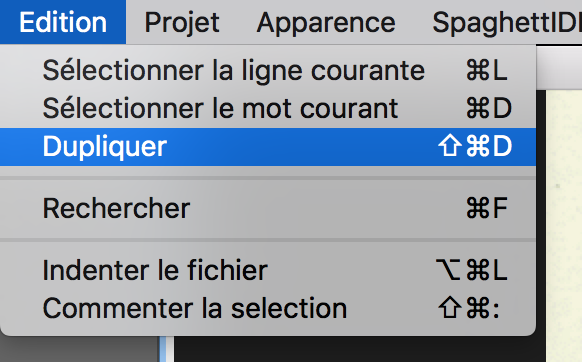
\includegraphics[scale=0.8]{images/imgs_edit/utilisation_duplication}
			\caption{Action du menu permettant de dupliquer}
		\end{center}
	\end{figure}


	\begin{figure}[h!]
		\begin{center}
			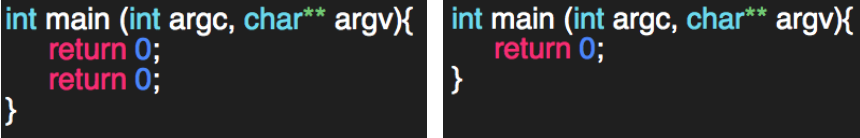
\includegraphics[scale=0.8]{images/imgs_edit/resultat_duplication}
			\caption{Résultat de l'utilisation de la fonction permettant de dupliquer}
		\end{center}
	\end{figure}

	\newpage
\subsection{Recherche}

	Pour la recherche dans le document, nous avons decidés d'ajouter une boite de dialogue permettant d'entrer le texte à rechercher. Pour cela nous avons créé une classe SearchDialog (héritant de QDialog), lors de l'affichage de cette boite de dialogue nous utilisons la méthode \textbf{exec}, qui rend impossible l'interaction avec la fenetre en arrière plan tant que la boite de dialogue est ouverte.

	Cette boite de dialogue nous permer de taper le texte à rechercher, de choisir si on recherche en avant ou en arrière, mais aussi si on veut être sensible à la case.

	\begin{figure}[h!]
		\begin{center}
			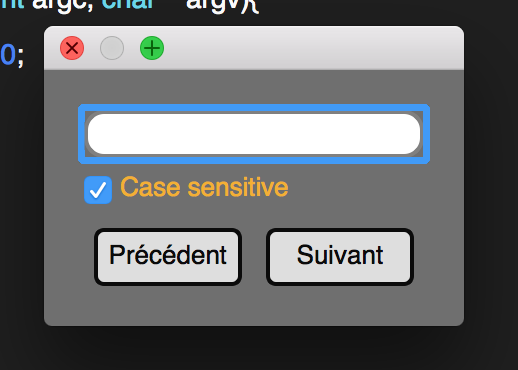
\includegraphics[scale=0.8]{images/imgs_edit/boite_dialog_recherche}
			\caption{Boite de dialogue relative à la recherche}
		\end{center}
	\end{figure}

	Pour la recherche on utilise la méthode \textbf{find} de notre objet Editeur. Cette méthode prend en paramètre le texte à rechercher, suivi de différents drapeaux. Dans notre cas nous utilisons le drapeau permettant d'exécuter la rechercher en arrière et le drapeau permettant de faire la recherche en étant sensible à la case (respectivement les drapeaux \textbf{QTextDocument.FindBackward} et \textbf{QTextDocument.FindCaseSensitively})

	\begin{figure}[h!]
		\begin{center}
			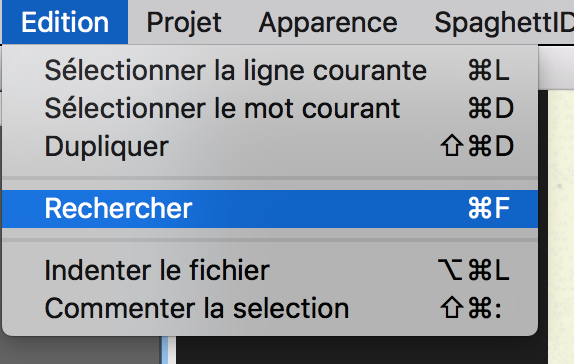
\includegraphics[scale=0.8]{images/imgs_edit/utilisation_rechercher}
			\caption{Action du menu permettant de rechercher}
		\end{center}
	\end{figure}

	\begin{figure}[h!]
		\begin{center}
			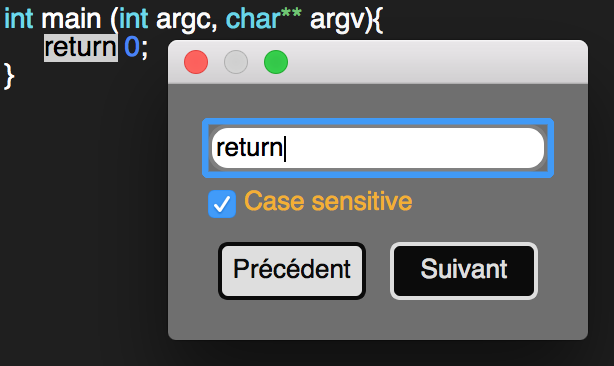
\includegraphics[scale=0.8]{images/imgs_edit/resultat_rechercher}
			\caption{Résultat de l'utilisation de la fonction permettant de rechercher}
		\end{center}
	\end{figure}
	\newpage

\subsection{Indentation du fichier}

	Pour l'indentation du document, nous allons changer son contenu (ajout/retrait de tabulation) nous devons donc stocker la position courante du curseur (grâce à la méthode \textbf{blockNumber} de l'objet QTextCursor). Par la suite on recupère le contenu du document grâce à la méthode \textbf{toPlainText} de l'objet Editeur. On créé une variable \textbf{indent\_level}, qui contient le niveau courant d'indentation, puis on parcourt toutes les lignes de notre document, si la ligne contient le charactère "\}", on retire 1 au niveau d'indentation puis on change la ligne pour ajouter au debut de cette dernière \textbf{indent\_level} fois une tabulation, puis on ajoute 1 au niveau d'indentation si la ligne contient "\{".
	Pour finir on defini le nouveau texte ainsi obtenu comme texte de notre document avec la méthode \textbf{setPlainText} et on replace le curseur au bon endroit.

	\begin{figure}[h!]

		\begin{center}
			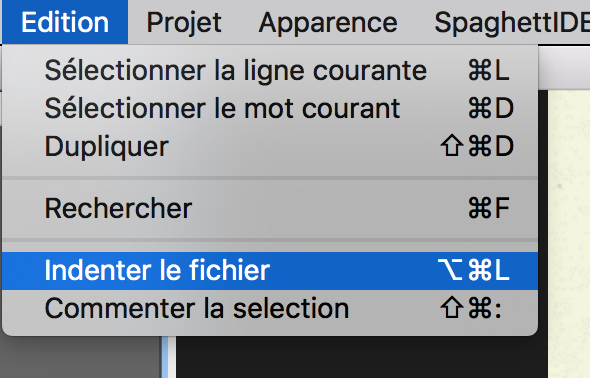
\includegraphics[scale=0.8]{images/imgs_edit/utilisation_indentation}
			\caption{Action du menu permettant d'indenter le fichier}
		\end{center}
	\end{figure}

	\begin{figure}[h!]
		\begin{center}
			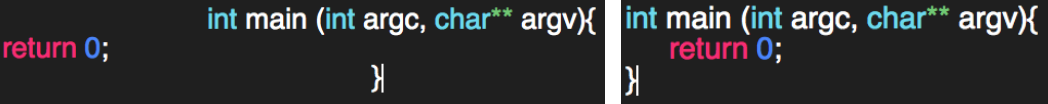
\includegraphics[scale=0.8]{images/imgs_edit/resultat_indentation}
			\caption{Résultat de l'utilisation de la fonction permettant d'indenter le fichier}
		\end{center}
	\end{figure}

\subsection{Commenter la sélection}

	De la même façon que pour la duplication du texte, nous avons séparé cette action en deux cas, soit du texte est sélectionné soit rien n'est sélectionné.
	Dans le cas ou du text est sélectionné nous commenterons seulement à partir du debut de la selection. Si plusieurs lignes sont selectionnées elles seront évidemment toutes commentées. Si il n'y a pas de texte sélectionné, on commente la ligne courante.

	Dans un premier temps, comme pour la duplication, si rien n'est selectionné on sélectionne la ligne courante, puis on sauvegarde le texte sélectionné que l'on recupère grâce à la méthode \textbf{selectedText}, puis on supprime le texte sélectionné avec la méthode \textbf{removeSelectedText}. Pour savoir si le texte est deja commenté, nous parcourons toutes les lignes, si une des lignes ne commence pas par "//" la sélection est considérée comme non commenté. Par la suite nous parcourons chaque ligne du texte puis pour chaque ligne nous ajoutons/retirons les charactères "//" en fonction de si le texte et oui ou non déjà commenté.

	Puis on ajoute le texte ainsi modifié à notre document en utilisant la méthode \textbf{insertText} (de l'objet QTextCursor).

	\begin{figure}[h!]

		\begin{center}
			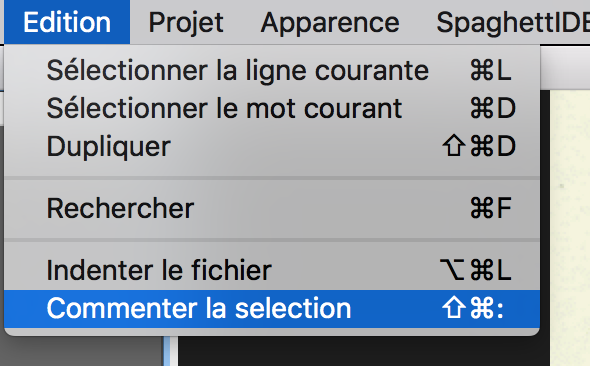
\includegraphics[scale=0.8]{images/imgs_edit/utilisation_commentaire}
			\caption{Action du menu permettant de commenter le fichier}
		\end{center}
	\end{figure}

	\begin{figure}[h!]
		\begin{center}
			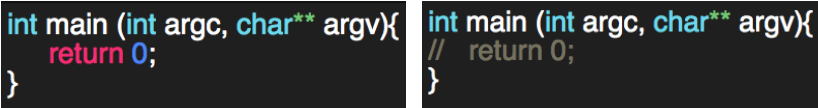
\includegraphics[scale=0.8]{images/imgs_edit/resultat_commentaire}
			\caption{Résultat de l'utilisation de la fonction permettant de commenter le fichier}
		\end{center}
	\end{figure}
	
\subsection{Les snippets}
	
	\subsubsection{Les snippets : explication}

		Les snippets sont des bouts de code qui sont réutilisables d'un projet à un autre (comme les conditions, les boucles et les définitions de fonction par example). Dans notre IDE nous utilisons des mots clés que l'on associes à ces bouts de code. Lorsque l'on tape un des mots clés puis que l'on presse la touche \textbf{tabulation}, le mot clé est remplacé par le bout de code qui correspond.

	\subsubsection{Intergration des bouts de code dans l'IDE}

		\paragraph{Utilisation du JSON}

			Pour l'intégration des snippets dans l'IDE, nous avons utilisés des fichier JSON, qui contiennent des dictionnaires avec comme clé le mot clé qui correspond au bout de code et en valeur le dit bout de code, suivit de nombre de ligne de le cursor doit remonter, puis le nombre de charactère char que le cursor doit parcourir vers la droite pour être à l'emplacement voulu. De plus nous avons un fichier JSON par language (C, python, etc ... )

			\begin{figure}[h!]
				\begin{center}
					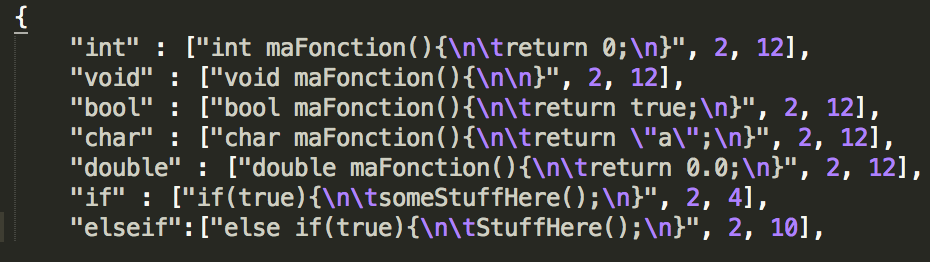
\includegraphics[scale=0.7]{images/exempleJSON}
					\caption{Extrait du fichier JSON pour le language C}
				\end{center}
			\end{figure}

		\paragraph{Connection entre le JSON et l'IDE}

			Pour capturer l'appuie sur la touche \textbf{tabulation}, nous utilisons le méthode \textbf{keyPressEvent} de notre classes \textbf{Editeur}. Cette méthode est appelée à l'appuie sur une des touches du clavier. Par la suite, si la touche est la touche \textbf{tabulation}, nous parsons le JSON pour avoir touts les couples mot clé - bout de code. Puis en fonction du mot placé au niveau du curseur, on le remplace ou non par le bout de code correspondant.

			\begin{figure}[h!]
				\begin{center}
					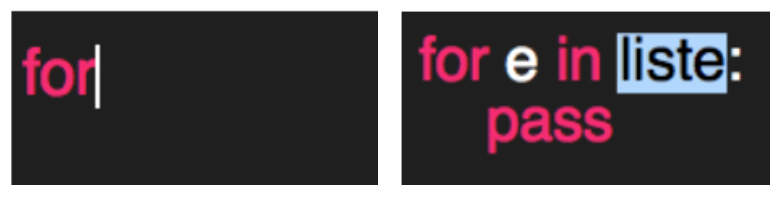
\includegraphics[scale=0.7]{images/exampleFor}
					\caption{Exemple d'utilisation des snippets avec une boucle for en Python}
				\end{center}
			\end{figure}

	
\section{Traitement des projets}

	\subsection{Import d'un projet}
	
	\subsection{Informations d'un projet}
	
	
\section{Fichier de configuartion XML}


\section{Compilateur}

	\subsection{Compilateurs utilisés}

		Pour notre IDE, nous avons utilisés le compilateur \textbf{GCC}, pour compiler les projets de type \textbf{C}. Mais nous utilisons aussi les interpréteur de python afin d'interpréter les projets de type \textbf{Python}. Par la suite, pour chaque nouveaux languages il nous suffit d'utiliser le bon compilateur ou le bon interpréteur.
		
	\subsection{Integration de \textbf{GCC} à notre IDE}

		Pour utilisé \textbf{GCC} avec notre IDE nous avons créé une fenêtre de configuration afin de permettre à l'utilisateur de choisir la configuration adéquate à la compilation de son projet.

			\begin{figure}[h!]
				\begin{center}
					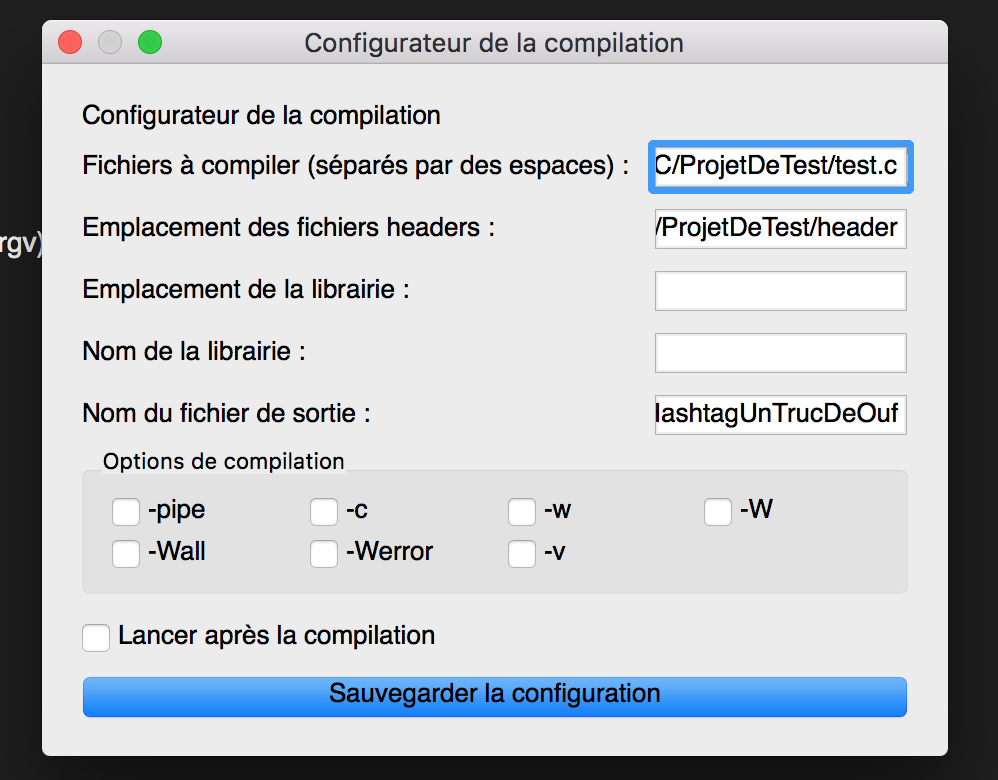
\includegraphics[scale=0.7]{images/fenCompEx}
					\caption{Fenêtre de configuration de GCC}
				\end{center}
			\end{figure}

		Par la suite, chaque information de cette fenêtre est convertie en une chaîne de caractère du type : 

		gcc /Users/theosarrazin/workplaceC/ProjetDeTest/test.c  -I /Users/theosarrazin/workplaceC/

		ProjetDeTest/header -o MonExecutable

		Cette chaîne de caractère est stockée dans le fichier XML de configuration du projet.

		Par la suite on exécute cette ligne de commande, puis on récupère sur la sortie d'erreurs les eventuelles erreurs afin de pouvoir les afficher à l'utilisateur après les avoir parsé pour avoir un bon formatage.

		\newpage

			\begin{figure}[h!]
				\begin{center}
					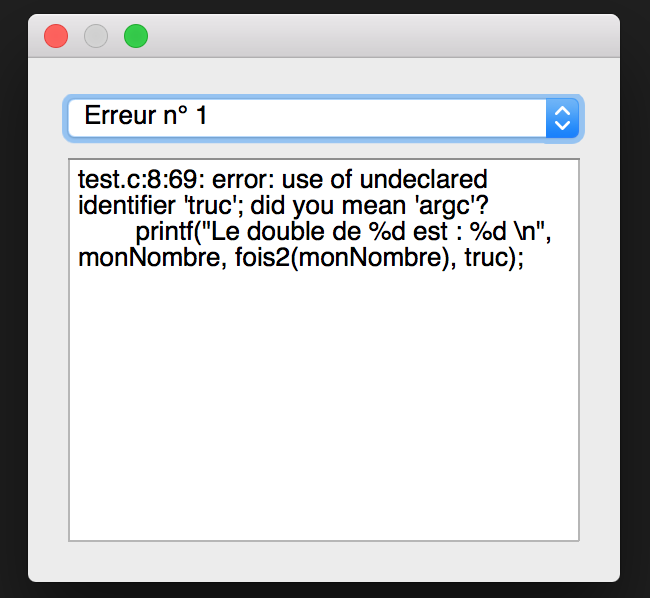
\includegraphics[scale=0.7]{images/fenErreurEx}
					\caption{Affichage des erreurs de GCC dans l'IDE}
				\end{center}
			\end{figure}

		Pour la partie interpréteur la demarche est identique. 


\section{Inspecteur d'éléments}

	Lorsqu'un document est ouvert, nous avons la possibilité d'afficher l'inspecteur d'éléments. Pour cela, nous avons le bouton "Navigateur" sous le navigateur de fichiers, et lorsque l'on clique dessus, on affiche l'inspecteur à la place. De même si on re-clique dessus, on ré-affiche le navigateur.
	
	\begin{figure}[h!]
		\begin{center}
			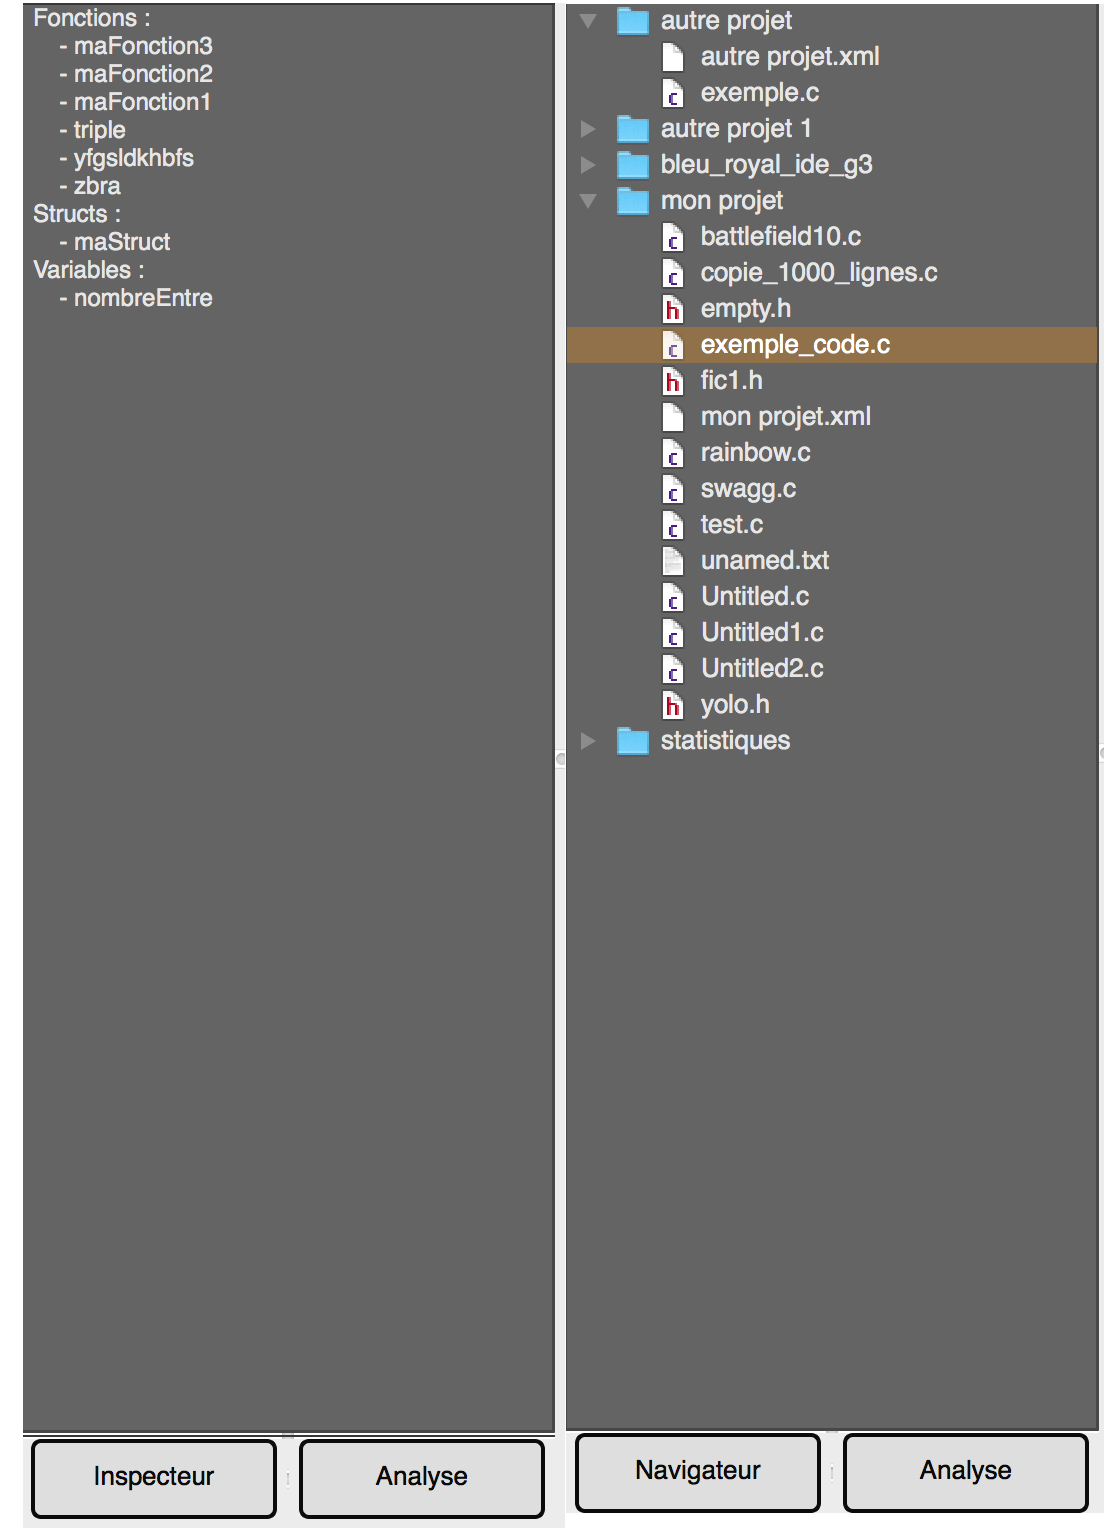
\includegraphics[scale=0.5]{images/insp_nav.png}
			\caption{Respectivement l'inspecteur et le navigateur de fichiers sont affichés}
		\end{center}
	\end{figure}
	
	Au niveau du code, le navigateur de fichiers est créé à l'aide d'un QTreeView (comme au premier semestre), et il est remplacé par un QTextEdit qui constitue l'inspecteur lorsqu'on clique sur le bouton.\\
	
	On affiche dans l'inspecteur toute la structure du code grâce au logiciel Yacc, qui peut nous renvoyer des listes contenant pour un fichier :
	
	\begin{itemize}
		\item Ses variables
		\item Ses fonctions
		\item Ses struct (en C) ou ses Class (en Python)\\
	\end{itemize}
	
	Lorsque l'on clique sur un élément par exemple un nom de variable, cette variable est sélectionné dans le document courant.

\section{Personnalisation des raccourcis}

	Dans le menu de notre IDE, vous avez pu remarquer qu'à côté de certaines options, il y avait des raccourcis que nous avions choisis en fonction de ce qui nous semblait être le mieux. Mais ces choix étaient personnels, et tous les membres du groupe n'approuvant pas certains choix, nous avons décidé de les rendre personnalisables.

	\subsection{Partie interface}

	Nous avons trois menus dans lesquels il y a des raccourcis. Ainsi, nous avons décidé de créer un fichier "racc\_defaut.json" qui contient un dictionnaire ayant pour clefs le noms de ces trois menus, et comme valeurs d'autres dictionnaires qui ont pour clefs les noms des fonctionnalités et comme valeurs une chaîne de caractères représentant le raccourci.

\begin{center}
	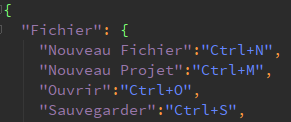
\includegraphics[scale=0.5]{images/imgs_racc/ex_1.png}\\
	Ici, un aperçu du fichier "racc\_defaut.json".
\end{center}

	Nous pouvons donc conserver tous les raccourcis de base et en proposer dès le lancement de l'IDE, au lieu de forcer l'utilisateur à en définir. Il peut donc choisir, via le menu "Fichier", dans le sous-menu "Paramètres", l'option Raccourcis, qui modifiera le fichier "racc\_utilisateur.json" créé lors du lancement de l'IDE si celui-ci n'existait pas déjà.\\

	Cliquer sur cette option lui ouvrira une nouvelle fenêtre (une QDialog), dans laquelle trois onglets (des QTabWidget) seront disponibles. Ces trois onglets correspondent aux trois menus qui contiennent des raccourcis. Dans ces onglets, des lignes de saisies (des QLineEdit) seront apparentes permettront à l'utilisateur de rentrer ses propres raccourcis. Nous avons mis les raccourcis de base en fond pour que l'utilisateur ait un modèle. Cette interface est complétée par deux boutons, l'un qui valide les raccourcis et l'autre qui les remet à zéro, c'est-à-dire qu'il modifie les valeurs contenues dans le fichier "racc\_utilisateur.json",  et les remplace par les valeurs contenues dans le fichier "racc\_defaut.json".

\begin{center}
	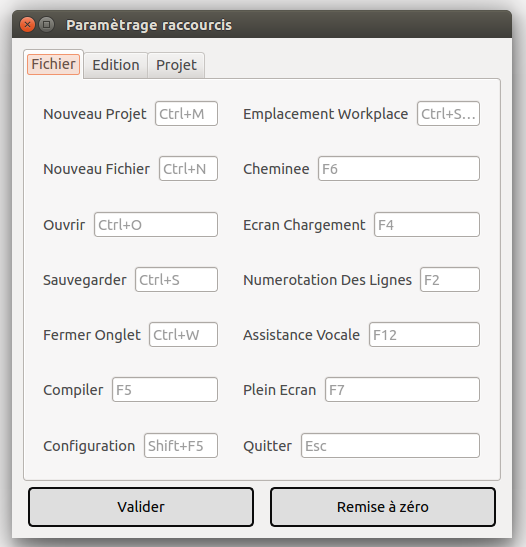
\includegraphics[scale=0.4]{images/imgs_racc/ex_2.png}\\
	Un aperçu de la fenêtre permettant la modification des raccourcis.
\end{center}

	\subsection{Partie modification}

En ce qui concerne la modification des raccourcis, il est possible de d'écrire tout ce que l'on veut dans les lignes de saisies. C'est lorsque l'on clique sur le bouton valider que la fonction qui valide un raccourci va être appelée. Ainsi, certaines combinaisons de touches ne sont pas permises, telles que "M+Shift+Ctrl". Nous avons aussi décidé de faire en sorte que si l'utilisateur écrit quelque chose de ce style : "Ctrl+Shift+JHGFFUTRF", on écrive dans le fichier "racc\_utilisateur.json" : "Ctrl+Shift+J".

\section{Cache des documents}

	\subsection{Utilité du cache}

		Afin de pouvoir faire de la coloration, nous avons utilisés \textbf{Lex} mais pour les fichiers de plusieurs 100\up{ène} de lignes \textbf{Lex} prend plusieurs secondes pour nous donner la listes des tokens du fichier. Nous avons donc décidé d'utiliser un fichier de cache afin de ne pas utiliser \textbf{Lex} pour colorer des lignes que nous avons déjà coloré de manière ultérieure.

	\subsection{Intégration du cache dans l'IDE}

		Pour le cache, nous avons décidé d'utiliser un fichier JSON pour l'enregistrer. Le fonctionnement est assez simple la clé est le bout de code que l'on donne à \textbf{Lex} et la valeur est la réponse de ce dernier. Par la suite il nous reste plus qu'à utiliser les valeurs du fichier JSON à la place de \textbf{Lex}

			\begin{figure}[h!]
				\begin{center}
					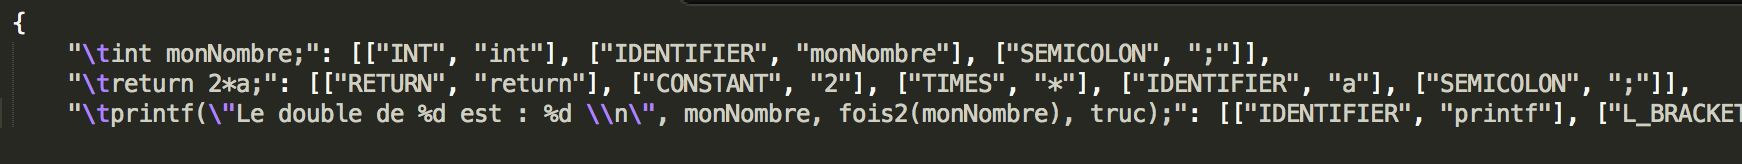
\includegraphics[scale=0.5]{images/exempleJsonCache}
					\caption{Extrait d'un JSON contenant le cache}
				\end{center}
			\end{figure}

		Grâce au cache nous avons un gain de temps considérable sur l'ouverture des documents.
		
		Nous pouvons que 2 fonctions existent, l'une vide le cache du projet courant et l'autre vide tout le cache. 

\section{Nouvelles grammaires}

	\subsection{Grammaire Arithmétique}

		\subsubsection{Lex}
			
			Comme nous avons pu le voir, les regles de lex sont définis par des tokens, chaques tokens étant associés à un expression régulière. 

			\paragraph{Les tokens}

				Dans le cadre d'un grammaire arithmétique nous avons besoin de différents tokens : 
				\begin{itemize}
					\item Number : le token qui va reconnaitre les nombres
					\item Plus : le token qui va reconnaitre le signe +
					\item Minus : le token qui va reconnaitre le signe -
					\item Times : le token qui va reconnaitre le signe *
					\item Divide : le token qui va reconnaitre le signe /
					\item LParen : le token qui va reconnaitre la parenthèse gauche
					\item RParen : le token qui va reconnaitre la parenthèse droite
				\end{itemize}

				Pour être reconnnu par Lex ces tokens sont stockés dans un tuple \textbf{tokens} 

			\paragraph{Les expressions régulières}

				A chacun des tokens précédents, nous devons associer une expression régulière pour que Lex puisse reconnaitre les tokens.
				Pour cela, nous devons simplement créer une variable de la forme t\_NomDuToken, est qui prend comme valeur l'expression régulière à associer à ce token.

				Pour le token Number, nous utilisons l'expression suivante : \textbf{\"\\b+\"}, le \textbf{\"\\b\"} signifiant n'importe quel chiffre compris entre 0 et 9 de plus le \textbf{+} signifie répété une ou plusieur fois. En effet un nombre est une suite de chiffre.

				Pour les six autres tokens, nous utilisons simplement le signe qui doit correspondre au token (+ pour le token Plus, - pour le token Minus, etc...)
			
				\begin{figure}[h!]
					\begin{center}
						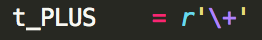
\includegraphics[scale=1]{images/exp_regex}
						\caption{Exemple de création d'une expression régulière}
					\end{center}
				\end{figure}


			\paragraph{Fonctions et variables supplémentaires}

				De plus, pour l'utilisation de Lex, nous pouvons définir une variable \textbf{t\_ignore} qui va preciser les éléments à ne pas prendre en compte, dans notre cas la variable vaut \textbf{" \t"}, nous ignorons donc les espaces et les tabulations.

				Nous pouvons aussi définir une fonction \textbf{t\_newline(t)}, qui prend un token en paramètre et qui va être utilisée pour matcher tous les retours à la lignes grâce à l'expression régulière \textbf{\"\\n+\"}, de plus cette fonction va ajouter pour chaque ligne trouvé 1 à l'attribut \textbf{lineno}, qui contient le nombre de lignes.

				Pour finir un autre fonction peut être utilisée, la fonction \textbf{t\_error(t)}, qui prend elle aussi on token en paramètre et qui va être appelée par le lexer à chaque token non reconnue par notre lexer. Cette fonction va afficher un message d'erreur puis ignorer le token grâce à l'instruction \textbf{t.lexer.skip(1)}, t étant le token courrant grâce au quel on recupère le lexer. 

		\subsubsection{Yacc}

			\paragraph{Création de la grammaire}

				Pour fonctionner Yacc à besoin de différentes règles de grammaires, chaques règles definissants comment peuvent s'"assembler" les différents tokens reconnus pour Lex.

				Pour definir des règles nous devons créer des fonctions nommer de la façons suivante : \textbf{p\_NomDeLaRegle}. Cette fonction doit contenir une docstring definissant les regles à respecter.

				\begin{figure}[h!]
					\begin{center}
						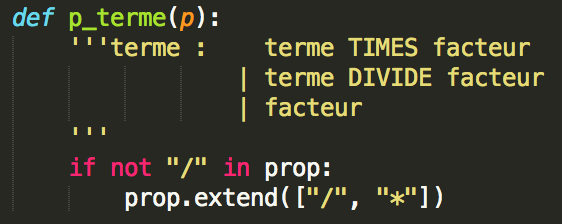
\includegraphics[scale=1]{images/exp_grammaire_yacc}
						\caption{Exemple d'une règle de grammaire de Yacc}
					\end{center}
				\end{figure}

				Voici nos différentes règles : 
				\begin{itemize}
					\item expression : correspond à une somme/soustraction de deux expressions. Une expression pouvant aussi être terme.
					\item terme : correspond à une multiplication/division de deux termes. Un terme pouvant aussi être un facteur.
					\item facteur : correspond à un nombre, une expression entre parenthèse ou - un facteur.
				\end{itemize}

				De plus, chacune de ces fonctions ajoute des propositions à une variable \textbf{prop} afin de les afficher par la suite dans notre IDE.

			\paragraph{Création du parser}

				Par la suite, nous devons appliquer nos règles sur du contenu, pour cela nous avons créés une fonction \textbf{parse}, qui prend en paramètre le code à parser. Par la suite, cette fonction créée le lexer (en faisant appelle à Lex), puis créée le parser (en faisant appelle à Yacc), pour finir elle revoit les listes des propostions afin de pouvoir les ajouter à les listes des propostions de notre IDE.
	
	\subsection{Grammaire Python}

		\subsubsection{Création de la grammaire}

			Dans un premier temps, nous avions commencé à rédiger une grammaire pour Python. Cependant nous avons rencontré plusieurs problèmes, notamment le fait qu'il n'est pas possible d'avoir des tokens imbriqués les uns dans les autres rendant ainsi les expressions régulière de \textbf{Lex} bien trop complèxe. De plus la gestion de l'indentation n'était pas facile. En effet \textbf{PLY} ne peut pas analyser l'indentation par ces grammaires, il nous faut donc révalider chacun des tokens identifiés par \textbf{Lex} dans un second temps. Chose qui n'est pas simple à faire avec la librairie \textbf{Ply}. Voila donc pourquoi nous avons décidé d'utiliser la librairie \textbf{PlyPlus}

		\subsubsection{Utilisation de la librairie PlyPlus}

			Pour pallier aux problèmes précédents, nous avons donc choisi d'utiliser la librairie \textbf{PlyPlus}. Cette librairie ce base sur la librairie \textbf{Ply} sur laquelle nous avons travaillé jusqu'à présent, il nous a donc était simple d'ajouter \textbf{PlyPlus} à notre projet. \textbf{PlyPlus} a plusieurs avantages, dont notament le fais d'avoir un système de grammaire totalement différent de \textbf{Ply}, nous permettant ainsi de résoudre les problèmes cités auparavant. Ce ne sont pas les seuls avantages de \textbf{PlyPlus}, en effet il nous permet aussi de sélectionner très simplement un type d'élément (le nom des fonctions ou des classes présentent par exemple) rendant ainsi possible leur coloration. De plus \textbf{PlyPlus}, vient avec une grammaire python et un post-analyseur syntaxique permettant ainsi de traiter l'indentation du fichier. 

	
\section{Langue du système en Anglais}

\section{Ajouts bonus}

	


\end{document}